\documentclass[12pt]{article}
\usepackage[left=1.5cm,right=1.5cm, top = 2cm, bottom = 2cm]{geometry}
\usepackage{graphicx}
\usepackage{natbib}
\usepackage{hyperref}
\usepackage{todonotes}
\usepackage{booktabs}
\usepackage{amssymb}
\usepackage{amsmath}

\newcommand{\sd}{s}
\newcommand{\mean}{\bar{y}}

\usepackage{caption}
\captionsetup[table]{name={{\footnotesize Table}}}
\usepackage{caption}
\captionsetup{font=footnotesize}

\begin{document}

\title{A statistical assessment of influenza intensity thresholds from the moving epidemic and WHO methods}
\author{Johannes Bracher$^{1, 2}$, Jonas M. Littek$^1$}
\date{18 June 2024\\ \medskip \small
$^1$Karlsruhe Institute of Technology (KIT), Institute of Statistics\\
$^2$Heidelberg Institute for Theoretical Studies (HITS), Computational Statistics Group\\ \medskip
Email address for correspondence:\\ \url{johannes.bracher@kit.edu}\\ % \medskip
}

\maketitle


\abstract{
\begin{quote}
Monitoring of influenza activity is a key task of public health agencies around the world. Intensity thresholds serve to retrospectively classify season peak intensity and to compare current influenza activity to past peak values. The resulting classifications into low, medium, high or very high intensity inform national-level risk assessment and planning. Moreover, they feed into international summary reports. Two common thresholding approaches, recommended in dedicated WHO guidelines, are the moving epidemic method (MEM) and the WHO method. In both approaches, thresholds correspond to quantiles of a normal distribution fitted to a set of historical observations. While an extensive literature on applications of these methods exists, their statistical properties have not been assessed systematically. In this paper we study them analytically and in a simulation study based on re-sampling of data from French influenza surveillance. Moreover, extensions to account for small sample sizes and secular trends are described. Under the default settings, both the MEM and WHO method on average classify more seasons than intended as high or very high intensity. Combining characteristics of both and adding a small-sample correction, better-calibrated thresholds can be achieved. Even these, however, have modest sensitivity and positive predictive values. This concerns especially thresholds for very high intensity.
\end{quote}
}

\bigskip

\begin{quote}
\textbf{Keywords:} calibration, influenza intensity threshold, moving epidemic method, predictive quantile, re-sampling, WHO method.
\end{quote}

\newpage


\section{Introduction}
\label{sec:introduction}

Influenza is a major public health threat and monitoring of influenza activity is a central task of health authorities around the world. To strengthen and standardize monitoring in the aftermath of the 2009 influenza H1N1 pandemic, the World Health Organisation (WHO) developed recommendations on severity assessment during seasonal and pandemic outbreaks. According to the PISA guidelines (\textit{Pandemic Influenza Severity Assessment}, \citealt{WHO2014}), severity is defined in terms of three dimensions. \textit{Transmissibility} refers to how many people become ill and is measured e.g., via weekly case numbers of influenza-like illness (ILI) or the percentage of such cases among all consultations by general practitioners. \textit{Severity} is commonly assessed by ratios of recorded deaths and hospitalizations or hospitalizations and cases. Lastly, \textit{impact} is measured e.g., by weekly case numbers of severe acute respiratory disease (SARI) or admissions to intensive care units.

A key role in the WHO PISA guideline is taken by influenza intensity thresholds. For transmissibility and impact indicators, they represent a generic tool to classify the peak intensity of an influenza season in light of past peak values. Typically, classifications into \textit{low}, \textit{medium/moderate}, \textit{high} and \textit{very high/extraordinary} intensity are provided. The rationale is that
\begin{quote}
\textit{``about 50--60\% of the season peaks should be above the moderate threshold, $\pm 10\%$ above the high threshold and $\pm 2.5\%$ above the extraordinary threshold''} \citep[p.10]{WHO2017}.
\end{quote}
Similarly to the idea of a ``100-year-flood'' used to communicate hydrological risks \citep{Holmes2010}, the definition of high and very high intensity influenza season peaks thus implies that on average they occur every 10 and 40 years, respectively.

Intensity thresholds form part of monitoring procedures in numerous countries, contributing to national-level risk appraisal and planning; see e.g., \cite{CDC2024} on their use in the United States. In addition, intensity classifications feed into international situation assessments like the weekly \textit{WHO Influenza Update} (see e.g., \citealt{WHO2024}). In this context, they facilitate comparisons and summaries across countries and surveillance systems. In practice, two uses of thresholds can be distinguished \citep{CDC2024}:
\begin{itemize}
\item[(1)] In the aftermath of an influenza season, thresholds serve to classify its peak intensity. As an example, the top panel of Figure \ref{fig:maps} shows an assessment of the 2022/23 season by the US Centers for Disease Prevention and Control (CDC; \citealt{White2023}). In terms of influenza-associated outpatient visits, hospitalization rates, and deaths among children and adolescents, this season was judged as high intensity.
\item[(2)] During an influenza season, values of relevant indicators can be compared to intensity thresholds on a weekly basis. The resulting classification is relative to past peaks rather than typical values at a given time of the season. An illustration is provided in the bottom panel of Figure \ref{fig:maps}. This display, published by the European Centre for Disease Prevention and Control (ECDC), summarizes influenza activity across Europe in a stylized map with colour coding.
\end{itemize}

\begin{figure}[h!]
\begin{center}
\fbox{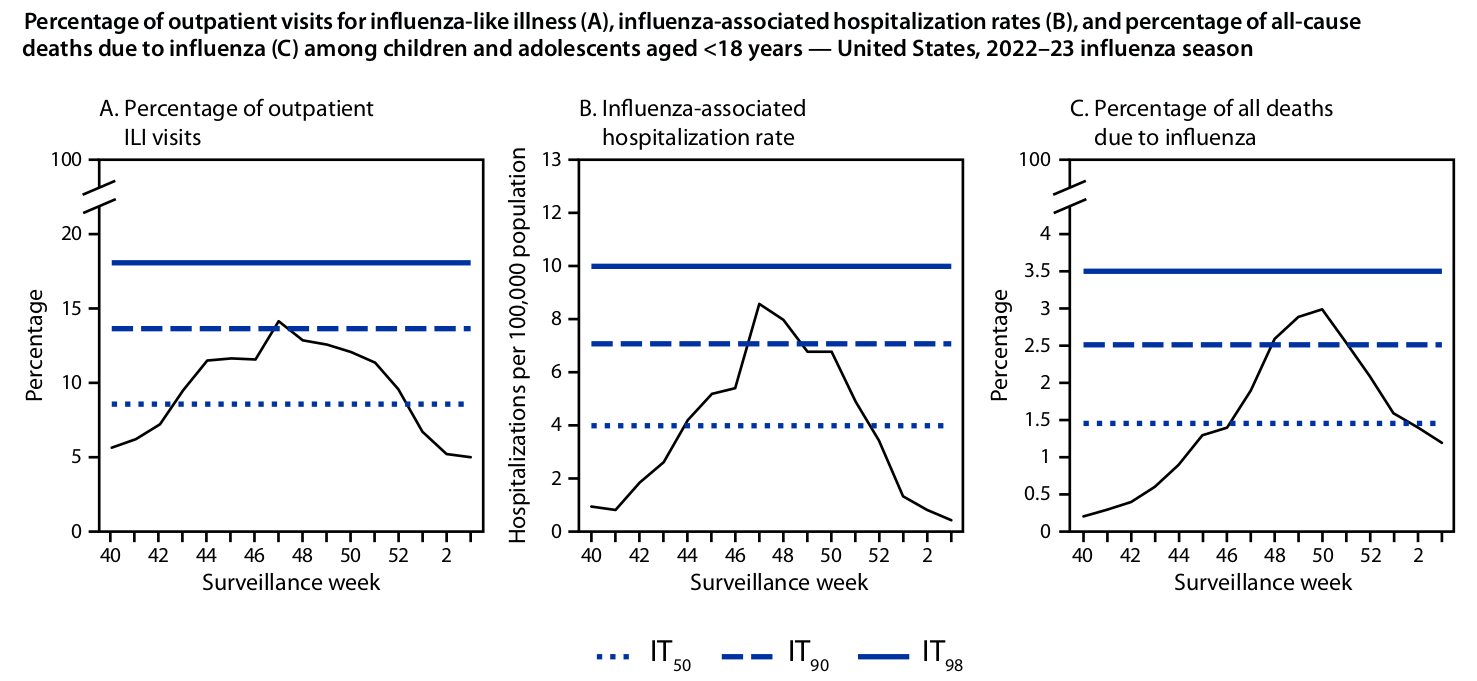
\includegraphics[width=0.85\textwidth]{figure/mmwr_with_heading.png}}

\medskip

\fbox{
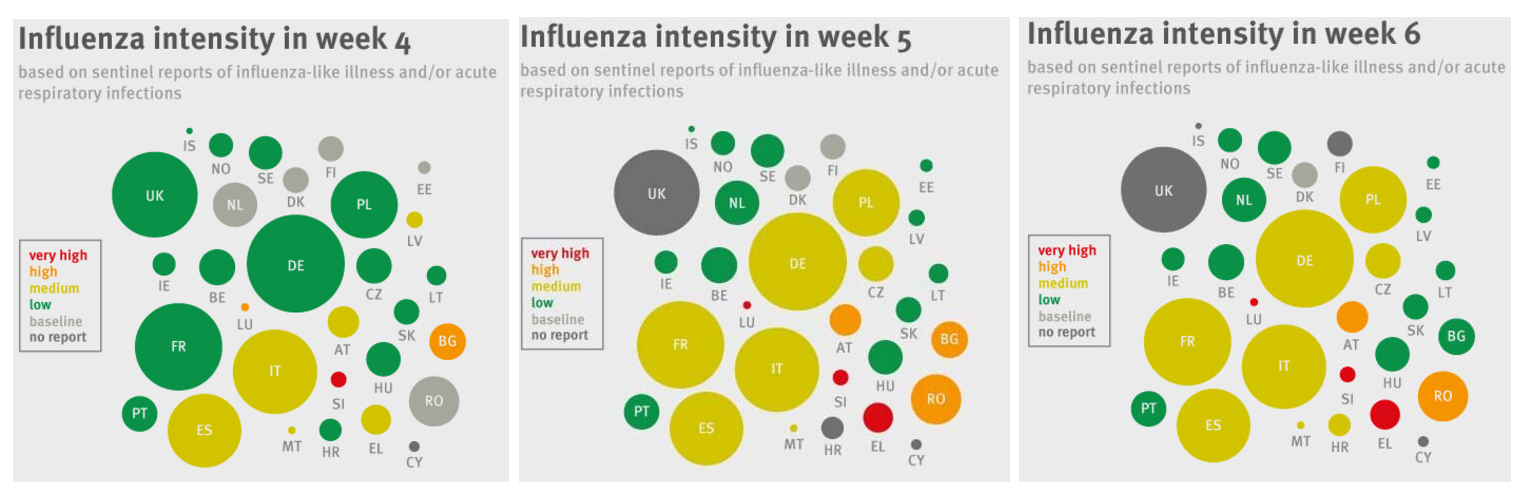
\includegraphics[width=0.845\textwidth]{figure/bubbles.png}}
\end{center}
\caption{Use of influenza intensity thresholds by public health agencies. Top: Retrospective classifications for the 2022/23 influenza season in the US by the CDC \citep{White2023}. Here, $\text{IT}_{50}, \text{IT}_{90}$ and $\text{IT}_{98}$ denote thresholds for medium, high and very high intensity. Bottom: Stylized influenza intensity maps published by ECDC in weeks 4 through 6, 2020. Copyright information is provided at the end of this article.
}
\label{fig:maps}
\end{figure}


\noindent Setting (1) is more closely aligned with the definition of thresholds in terms of nominal exceedance probabilities for new peak values, and the remainder of the article will focus on this task. We will return to setting (2) in the discussion. Note that we only address the question of peak intensity thresholds, but not baseline thresholds to determine the season onset \citep{Vega2013}; some analyses on these can be found in \cite{Pang2023}.

In the PISA guidelines \citep{WHO2017}, two statistical methods were recommended for influenza intensity thresholding. These are the \textit{moving epidemic method} (MEM; \citealt{Vega2015}) and the \textit{WHO method} \citep{WHO2014}, also referred to as the \textit{average curves method}. The former has also been recommended by ECDC (e.g., \citealt{ECDC2017}) and is used by the US CDC \citep{Biggerstaff2017}. As will be detailed in Section \ref{sec:definitions}, the WHO and MEM approaches bear important similarities and can be seen as variations of the same general approach. The two methods have been adopted by many public health agencies (see Section \ref{sec:review}). Their statistical properties, however, have not yet been studied. In the present work, we aim to close this gap and derive some recommendations for the computation of influenza intensity thresholds. We study the MEM and WHO methods and suggest extensions to account for small sample sizes and secular trends. We obtain some analytical results on their properties, complemented by simulation experiments based on re-sampling of routine surveillance data from France and the US. These indicate that using the default settings, both the MEM and the WHO method tend to produce too low thresholds. Consequently, the number of season peaks classified as high or very high intensity is higher than intended. The best-behaved thresholds are achieved by combining characteristics of the MEM and WHO methods, along with a correction for small sample sizes. Even this configuration, however, is characterized by modest sensitivity and positive predictive values unless data on many historical seasons are available. This concerns especially thresholds for very high intensity, which should thus be interpreted with care.

The remainder of the article is structured as follows. In Section \ref{sec:desirable_properties} we list desirable properties of a thresholding procedure, which will guide the discussion in the following. Section \ref{sec:definitions} provides definitions of the MEM and WHO methods, highlighting three differences between these otherwise similar approaches. Section \ref{sec:review} consists of an overview of published applications of the MEM and WHO methods, as well as some background on related disease monitoring methods. In Section \ref{sec:formalization_extension} we re-state the thresholding task as a statistical prediction problem and suggest some extensions to the methodology. This is followed by an examination of statistical properties of the methods in Section \ref{sec:analytical_results}. In Section \ref{sec:simulation} we conduct the simulation study before concluding with a discussion in Section \ref{sec:discussion}. Here we also provide practical recommendations on the different implementation choices.


\section{Desirable properties of thresholding methods}
\label{sec:desirable_properties}

We start by stating properties of a thresholding method which we consider desirable. These will guide the analyses in the remainder of the paper.

\begin{description}
\item \textbf{Calibration.} As stated in Section \ref{sec:introduction}, thresholds are defined in a statistical manner -- the respective thresholds should be exceeded by 60\%, 10\% and 2.5\% of season peaks. Threshold setting thus corresponds to determining predictive quantiles for future season peak values, and a major requirement is that these are \textit{calibrated}. We call a thresholding method calibrated if in the long run, the intended fractions of seasons are classified as low, medium, high and very high. If, for instance, a method flags new season peaks as very high intensity in considerably more than 2.5\% of the cases, this will hamper the usefulness of thresholds.
\item \textbf{Sensitivity and specificity.} In addition to classifying the intended fraction of seasons into the various categories, the individual classifications should be correct. Assuming there is an underlying stationary distribution of season peaks, a peak which is truly among the 2.5\%/10\%/60\% highest peaks should also be flagged as such (\textit{sensitivity}). Conversely, a peak which is not actually among the 2.5\%/10\%/60\% highest ones should not exceed the respective threshold (\textit{specificity}). These aspects, though, can only be assessed in theory and simulation studies, where the true intensity status can be determined based on the assumed distribution of peaks. In real-world applications, there is no ``gold standard'' to determine the true intensity level.
\item \textbf{Stability.} Estimated thresholds should not be overly variable. Ideally they would not fluctuate strongly around the corresponding quantiles of the true distribution of season peaks.
\item \textbf{Simplicity.} To ensure broad practical applicability, understanding the thresholding method and its parameters should not require advanced statistical training.
\item \textbf{Ease of practical application.} Methods should be straightforward to apply using well-documented and, ideally, open-source software packages.
\end{description}



\section{Definition of the MEM and WHO methods}
\label{sec:definitions}

While framed slightly differently in the respective documentations, the MEM and WHO methods are two special cases of the same general approach. We assume that thresholds are based on weekly values of a transmissibility or severity indicator (see Section \ref{sec:introduction}) from $m$ past seasons and applied to the ($m + 1$)-th season.  We denote the value for season $j$ and week $k$ by $x_{j, k}$, with more specific notation introduced below. Implicitly it is assumed that each season consists of just one wave without multiple peaks separated by longer time spans. This is typically the case in temperate, but not necessarily in tropical regions. Thresholds are then obtained via the following steps.

\begin{enumerate}
\item[(a)] \textbf{Smoothing of historical data} (optional): apply an $l$-week moving average to all historical seasons. If data are smoothed, we denote by $x^\text{raw}_{j, k}$ the raw observation from season $j = 1, \dots, m$, week $k = 1, \dots, 52$, and by
$$
x^\text{smo}_{j, k} = \frac{1}{l} \sum_{d = 0}^{l - 1} x^\text{raw}_{j, k - d}, \ \ k = l, \dots, 52
$$ the smoothed version. In the remainder of this description we denote whichever of $x^\text{raw}_{j, k}$ and $x^\text{smo}_{j, k}$ is used to compute thresholds by $x_{j, k}$.
\item[(b)] \textbf{Sorting:} Within each historical season $j = 1, \dots, m$ order all observations $x_{j, k}$ in decreasing order, denoting the $i$-th largest observation from season $j$ by $x^{(i)}_j$. More generally we will use the notation $^{(\cdot)}$ to denote an ordering of values, e.g., denoting by $x^{\text{raw}, (i)}_j$ the $i$-th largest unsmoothed incidence value from season $j$.
\item[(c)] \textbf{Selection of reference set:} Select the $n$ largest observations from each of the $m$ past seasons to construct a reference set $\mathcal{X} = \{x_j^{(i)}: j = 1, \dots, m; i = 1, \dots, n\}$.
\item[(d)] \textbf{Data transformation:} Apply a monotonically increasing transformation $y_j^{(i)} = f(x_j^{(i)})$ to all members of the reference set $\mathcal{X}$ to obtain a reference set $\mathcal{Y}$ of transformed values.
\item[(e)] \textbf{Fitting a normal distribution:} Assume that the transformed values in $\mathcal{Y}$ come from a normal distribution and compute estimates of its mean and variance,
\begin{align}
\begin{split}
\bar{y} & = \frac{\sum_{j = 1}^m\sum_{i = 1}^n y_j^{(i)}}{n\times m}\\
\sd^2 & = \frac{\sum_{j = 1}^m\sum_{i = 1}^n \left(y_j^{(i)}  - \bar{y}\right)^2}{n\times m - 1}.
\end{split}\label{eq:moments}
\end{align}
\item[(f)] \textbf{Computation of thresholds:} Define intensity thresholds on the transformed scale as quantiles of the normal distribution N$(\bar{y}, \sd^2)$, i.e.\ compute
\begin{equation}
\hat{q}_{Y, \alpha} = \bar{y} + z_\alpha \sd, \label{eq:def_q}
\end{equation}
with $z_\alpha$ the $\alpha$ quantile of the standard normal distribution. The $\hat{q}_{Y, \alpha}$ can be seen as estimates of quantiles $q_{Y, \alpha}$ of an underlying distribution of peak values. The default choices are
\begin{itemize}
\item[(i)] the 40th percentile $\hat{q}_{Y, 0.4} = \bar{y} - 0.25 \sd$ as the threshold for medium intensity;
\item[(ii)] the 90th percentile $\hat{q}_{Y, 0.9} = \bar{y} + 1.28 \sd$ as the threshold for high intensity;
\item[(iii)] the 97.5th percentile $\hat{q}_{Y, 0.975} = \bar{y} + 1.96\sd$ as the threshold for very high intensity.
\end{itemize}
As we will detail in Section \ref{subsec:reformulation}, we will moreover consider an alternative formulation based on the $t$-distribution,
\begin{equation}
\hat{q}_{Y, \alpha} = \bar{y} + t_{m\times n - 1, \alpha} \times \sqrt{1 + \frac{1}{m\times n}} \times s,
\label{eq:q_Y_t}
\end{equation}
with $t_{m\times n - 1, \alpha}$ the $\alpha$ quantile of the $t$ distribution with $m\times n - 1$ degrees of freedom.
\item[(g)] \textbf{Transformation of thresholds to the original scale:} Obtain thresholds on the original scale by applying the inverse transformation, i.e. for $\alpha = 0.4, 0.9, 0.975$ set% $\hat{q}_{X, 0.4} = f^{-1}(\hat{q}_{Y, 0.4})$, $\hat{q}_{X, 0.9} = f^{-1}(\hat{q}_{Y, 0.9})$, $\hat{q}_{X, 0.975} = f^{-1}(\hat{q}_{Y, 0.975})$.
$$
\hat{q}_{X, \alpha} = f^{-1}(\hat{q}_{Y, \alpha}).
$$
\item[(h)] \textbf{Application of thresholds:} The thresholds are applied to classify the peak value of the $(m + 1)$-th season. Depending on the exact specification, thresholds can be applied either to the raw peak value $x_{m + 1}^{\text{raw}, (1)}$ or the smoothed version $x_{m + 1}^{\text{smo}, (1)}$.
\end{enumerate}

\noindent The MEM and WHO methods are special cases of this procedure, see also Table \ref{tab:differences} and the graphical illustration in Figure \ref{fig:illustration}. In the MEM, no smoothing is applied and the default transformation $f$ is the natural logarithm.  \cite{Vega2015} recommend using $5 \leq m \leq 10$ seasons to ensure a recent data basis. The number of observations included per season is set to $n = 30/m$, rounded to the nearest integer (with a minimum value of $n = 1$). The total number $m \times n$ of historical observations is thus kept approximately fixed. This corresponds to the description by \cite{Vega2015} and the default settings of the R package \texttt{mem} \citep{Lozano2020}. The package, however, permits the user to choose $n$, $m$, and $f$, see Supplement B.1. We note that while \texttt{mem} does not currently allow for data smoothing using a moving average, some alternatives are available. Thresholds based on a $t$-distribution as in equation \eqref{eq:q_Y_t} were not implemented when the computations for this paper were run, and an independent custom function was used instead. In the meantime, however, this feature has been added to the development version of the \texttt{mem} package, see Supplement B.1.

The implementation of the WHO method in the publicly available \textit{WHO Average Curves} Shiny Web App \citep{WHO2023} likewise offers a lot of flexibility. Our description is based on the default settings as of June 2024 and the description in \cite{WHO2014}. Smoothing of data prior to the computation of thresholds is recommended, with a default of $l = 3$ (adapted from $l = 4$ in \citealt[p68]{WHO2014}). Subsequently, $n = 1$ observation per season is used and by default no transformation is applied to the reference set. If peak incidences vary strongly across seasons, a log transformation is recommended. At least $m = 3$ historical seasons are required, but it is noted that the ``accuracy of these thresholds should be expected to increase with the number of seasons of good quality data available'' \cite[p22]{WHO2023}. Thresholds are by default applied to unsmoothed new peak values. Thresholds based on a $t$-distribution are available, but they are not the default and as of June 2024 do not seem to take into account the factor $\sqrt{1 + 1/(m + n)}$ from equation \eqref{eq:q_Y_t}.


Both the inclusion of multiple observations per season in the MEM ($n > 1$) and the smoothing of data in the WHO method ($l > 1$) can be seen as attempts to base thresholds on more data than just one peak value per historical season. This is intended to make estimation more stable. The impact of these strategies on the resulting thresholds will be discussed in Section \ref{sec:analytical_results}.



\begin{table}[h]
\caption{Default settings of the moving epidemic and WHO methods. Both procedures are visualized in Figure \ref{fig:illustration}.}
\label{tab:differences}
\begin{center}
\footnotesize
\begin{tabular}{lll}
\toprule
& moving epidemic method & WHO Method \\
\midrule
smoothing of historical data & none & moving average, $l = 3$\\
number $n$ of observations used per season & $n = \max[\text{round}(30/m), 1]$ & $n = 1$\\
default transformation for reference set & natural logarithm & none\\
recommended number $m$ of historical seasons & $5 \leq m \leq 10$ & $m \geq 3$, more recommended\\
smoothing of new season peak & none & none\\
\bottomrule
\end{tabular}
\end{center}

\end{table}


\begin{figure}
\begin{center}
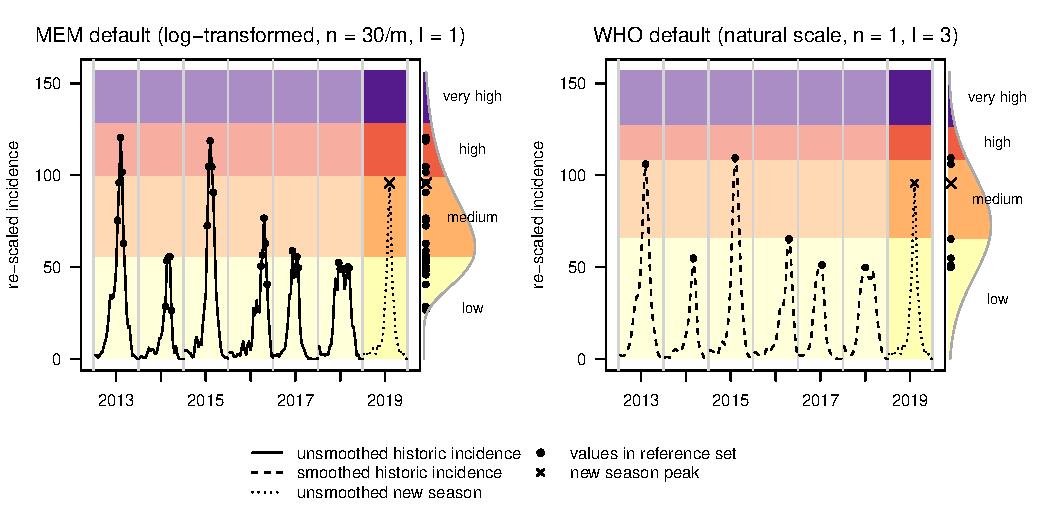
\includegraphics[width = 0.78\textwidth]{figure/illustration_mem_who.pdf}
\end{center}
\caption{Illustration of the MEM and WHO methods with their respective default settings, computed using $m = 6$ historical seasons (solid / dashed lines depending on whether smoothing is applied). These thresholds are applied to a seventh season (dotted lines, peak highlighted by a cross). Here, both methods classify the new season peak as medium intensity. Observations included in the reference set are highlighted by dots (with $n = 30/6 = 5$ for MEM, $n = 1$ smoothed values for WHO). The distribution fitted to the reference set is shown as a vertical density plot. Note that for the MEM this is a log-normal as the normal distribution is fitted to log-transformed values. The data used for illustration correspond to the years 2012--2019 from the French region of Grand Est, see Section \ref{subsec:data} and Figure \ref{fig:data}.}
\label{fig:illustration}
\end{figure}



\section{Related literature}
\label{sec:review}

\subsection{Use cases of the MEM and WHO method}


To improve our understanding of the settings in which the MEM and WHO methods are applied in practice we performed a literature search of articles published in English language and citing the papers \cite{Vega2015}, \cite{WHO2014} and \cite{WHO2017} until May 2023 (identified via \textit{CrossRef} and \textit{Google Scholar}). The results are summarized in Supplementary Table S1.

The large number of entries from the years 2019 and 2020 indicates that the MEM has quickly become a standard approach to set intensity thresholds for influenza and other respiratory diseases. The articles come from numerous countries and in many cases have been co-authored by representatives of national or regional public health agencies. In most analyses, threshold levels at the 40th, 90th and 97.5th percentile as in Section \ref{sec:definitions} are used. Variability with respect to the number $m$ of historical seasons included is considerable, with a range from 3 to 16. Consequently, the number $n$ of observations included per season ranges from two to ten. Only one paper \citep{Dahlgren2022} indicated a modification of the default setting $n = 30/m$  and used $n = 3$ with $m = 7$.

We only found six published applications of the WHO method, two of which provide a comparison to the MEM approach \citep{Rguig2020, Teeluck2021}. In most cases it is not documented whether smoothing was applied and which value was chosen for $l$. Several papers used the 95\% rather than 97.5\% quantile for the highest threshold.



\subsection{Related disease monioring methods}
\label{sec:related_literature}


There is a vast literature on monitoring tasks in infectious disease epidemiology and public health. Well-known approaches include Shewhart, cumulative sum (CUSUM, \citealt{Hoehle2008}) and exponentially weighted moving average (EWMA, \citealt{Steiner2010}) control charts. Time series methodology can likewise be employed, see e.g., \cite{Reis2003} for an application of ARIMA models. For a comprehensive account we refer the reader to the review aricles by \cite{Allevius2020}, \cite{Rigdon2015} and \cite{Unkel2012}. In the following we focus on two widely used approaches with close links to the MEM and WHO methods.

A simple Shewhart-type method is used by the US CDC as part of the \textit{EARS} system (Early Aberration Reporting, \citealt{Hutwagner2003}). Denote by $y_1, \dots, y_m$ the $m$ most recent values of a daily epidemiological indicator. An upper alarm threshold for a new observation $y_{m + 1}$ is given by
$$
U = \bar{y} + 3 \times s,
$$ 
where, similarly to equation \eqref{eq:moments} we set $\bar{y} = 1/m \times \sum_{j = 1}^m y_j$ and $s^2 = 1/(m - 1) \times \sum_{j = 1}^m (y_j - \bar{y})^2$. This closely resembles the WHO method, i.e., the procedure from Section \ref{sec:definitions} with $n = 1$ and $f$ the identity function. The multiplier 3 corresponds to $\alpha = 0.9987$. This approach was conceived as a ``drop -in'' surveillance method, i.e., a method to be used in the short term and based on little data. In practice, $m = 7$ observations are used to compute thresholds, which is similar to the typical number of historical seasons used in intensity thresholding.

The EARS approach can also be seen as an intercept-only linear regression model,
$$
Y_{t} = \beta_0 + \varepsilon_{t}, \ \ \ \ \varepsilon_t \sim \text{N}(0, \sigma_\varepsilon^2),
$$
with $\bar{y}$ and $s^2$ as estimators of $\beta_0$ and $\sigma_\varepsilon^2$. Indeed, regression-based approaches represent a flexible and general monitoring framework, compare Section 2 in \cite{Unkel2012}. Classic parametric approaches like the \textit{Serfling method} \citep{Serfling1896} are widely used, see e.g., \cite{Thompson2009} for an application to influenza mortality. Here, a regression model including time trends and sinusoidal functions for seasonality, say,
\begin{equation}
Y_{t} = \beta_0 + \beta_1 t + \beta_2 \sin(2\pi t / \omega) + \beta_3 \cos(2\pi t / \omega) + \varepsilon_t, \ \ \ \varepsilon_t \sim \text{N}(0, \sigma_\varepsilon^2),
\label{eq:serfling}
\end{equation}
is fitted to historical values $y_1, \dots, y_m$ spanning multiple seasons. The period of seasonal cycles is given by $\omega$, with $\omega = 52$ for weekly data and yearly seasonality. From the model fit predictive quantiles for a new value $y_{m + 1}$ are obtained, which serve as alarm thresholds. The equally popular \textit{Farrington method} is conceptually similar, but adapts to low-count settings via suitable data transformations \citep{Farrington1996} or count-valued response distributions \citep{Noufaily2013}. While technically a generalization of the EARS approach, the rationale of the Serfling and Farrington methods is somewhat different. As noted by \cite{Hutwagner2003}, the latter aim to detect deviations from past seasonal patterns while accounting for long-term trends. EARS, on the other hand, targets abrupt changes relative to the most recent observations.



\section{Statistical formalization and extension}
\label{sec:formalization_extension}

\subsection{Formulation as a prediction task}
\label{subsec:reformulation}

We now re-state the purpose and assumptions of the WHO and moving epidemic methods in statistical terms, denoting random variables by capital letters (e.g., $X_j^{(i)}$) and their realizations by lower-case letters (e.g., $x_j^{(i)}$). The goal of the thresholding exercise is to use data from seasons 1 through $m$ to obtain values $\hat{q}_{Y, \alpha}$ which shall be exceeded by a new transformed peak value $Y_{m + 1}^{(1)}$ with probabilities $(1 - \alpha) \in \{0.6, 0.1, 0.025\}$, respectively. The $\hat{q}_{Y, \alpha}$ can thus be seen as \textit{predictive quantiles} at levels $\alpha \in \{0.4, 0.9, 0.975\}$. Prediction of new realizations based on parametric assumptions and a set of previous observations is a well-studied problem; see e.g., \cite{Millard2013} on applications in environmental studies. We note that in \cite{WHO2014} and \cite{Vega2015} the thresholds are refered to as the upper ends of one-sided confidence intervals. This, however, is imprecise terminology as in the computations the standard deviation $\sd$ rather than the standard error $\sd/\sqrt{nm}$ is used (see documentation of the \texttt{mem} package and \citealt{WHO2014}, p.69).

Implicitly, both the WHO and the moving epidemic method assume that the elements of $\mathcal{Y}$ are independent and identically distributed draws from a Gaussian distribution, and that the new peak value $Y_{m + 1}^{(1)}$ comes from that same distribution. As we will examine different violations of this overall assumption, we state its various aspects in more detail. To this end denote by
\begin{equation}
\tilde{\mathbf{Y}}_j = (Y^{(1)}_j, \dots, Y^{(n)}_j)^\top\label{eq:Y_tilde}
\end{equation}
the random vector of the $n$ largest transformed incidence values from season $j$ in decreasing order. The set $\mathcal{Y}$ thus results from pooling $\tilde{\mathbf{Y}}_1, \dots, \tilde{\mathbf{Y}}_m$. We then distinguish the following assumptions.
\begin{itemize}
\item[\textbf{(H)}] It is assumed that the elements of $\tilde{\mathbf{Y}}_1, \dots, \tilde{\mathbf{Y}}_{m + 1}$ are \textit{homogeneous} in two ways.
\begin{itemize}
\item[\textbf{(HB)}] \textit{Between-season} homogeneity is assumed, meaning that the distribution of $\tilde{\mathbf{Y}}_j$ is the same for $j = 1, \dots, m + 1$. Time trends and changes in seasonal patterns are thus excluded.
\item[\textbf{(HW)}] Moreover, \textit{within-season} homogeneity is assumed in the sense that the elements $Y_j^{(1)}, \dots, Y_j^{(n)}$ of each vector $\tilde{\mathbf{Y}}_j, j = 1, \dots, m$ all follow the same distribution.
\end{itemize}
\item[\textbf{(I)}] Two \textit{independence} assumptions paralleling (HB) and (HW) are made.
\begin{itemize}
\item[\textbf{(IB)}] The vectors $\tilde{\mathbf{Y}}_1, \dots, \tilde{\mathbf{Y}}_{m + 1}$ are assumed to be independent. We thus do not allow for for correlations between subsequent seasons.
\item[\textbf{(IW)}] The elements $Y_j^{(1)}, \dots, Y_j^{(n)}$ within a vector $\tilde{\mathbf{Y}}_j$, i.e., the $n$ highest observations from the same season $j$, are assumed to be independent.
\end{itemize}
\item[\textbf{(N)}] It is assumed that the transformation $f$ leads to multivariate \textit{normality} of $\tilde{\mathbf{Y}}_j, j = 1, \dots, m$.
\end{itemize}
Whether assumptions (HB) and (IB) are reasonable is largely an empirical question. Assumptions (HW) and (IW), on the other hand, are almost inevitably violated if $n > 1$, as by construction $Y_j^{(1)} \geq Y_j^{(1)} \geq \dots \geq Y_j^{(n)}$. Technically, assumption (N) is likewise incompatible with this constraint, but may be helpful in practice.  For the time being we nonetheless accept all of the above assumptions and state standard theory on predictive quantiles in this setting. For large $m\times n$, the normal approximation
$$
\hat{q}_{Y, \alpha} = \bar{y} + z_\alpha \sd
$$
as in equation \eqref{eq:def_q} can be used. A common rule of thumb is to require $m \times n \geq 30$ (which seems to be the reasoning behind the MEM default setting $n = 30/m$). For small $m \times n$, however,
\begin{equation*}
\hat{q}_{Y, \alpha} = \bar{y} + t_{m\times n - 1, \alpha} \times \sqrt{1 + \frac{1}{m\times n}} \times s
\end{equation*}
as in equation \eqref{eq:q_Y_t} should be used (see e.g., \citealt{Preston2000}). The $t$-distribution with $m \times n$ degrees of freedom here accounts for the fact that the standard deviation $s$ needs to be estimated along with $\bar{y}$. As illustrated in Figure \ref{fig:illustration_t}, the predictive quantiles, and thus intensity thresholds, resulting from \eqref{eq:def_q} and \eqref{eq:q_Y_t} can differ substantially for small $m \times n$, with the latter leading to higher values for $\alpha = 0.9, 0.975$. We note that \cite{Allevius2020} have brought forward the same argument with respect to the EARS method.


\begin{figure}
\begin{center}
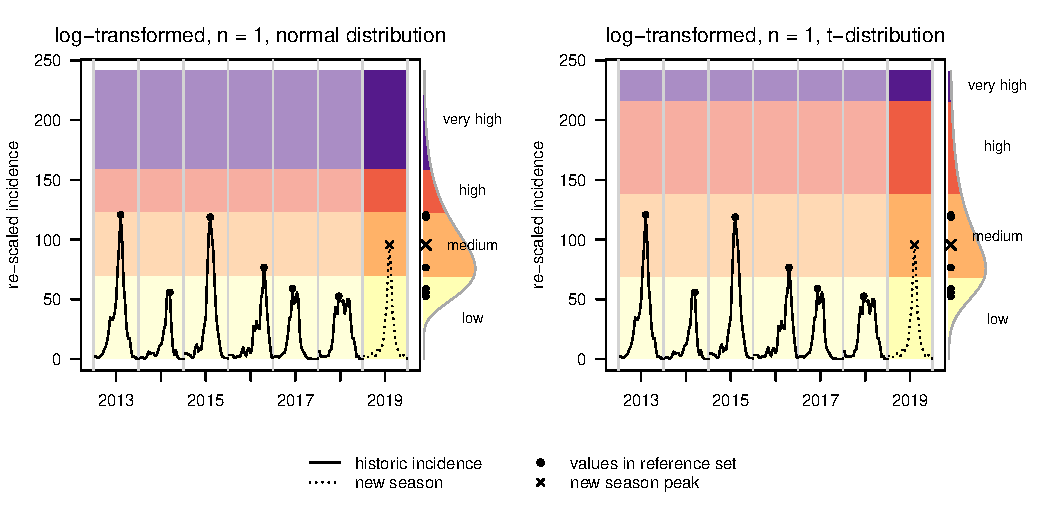
\includegraphics[width = 0.8\textwidth, trim={0 5mm 0 0},clip]{figure/illustration_t_normal.pdf}\vspace{-5mm}
\end{center}
\caption{Comparison of thresholds based on the normal and $t$-distribution (using $m = 6, n = 1$ and a log transformation). The data correspond to the years 2012--2019 from the French region of Grand Est, see Section \ref{subsec:data} and Figure \ref{fig:data}.}
\label{fig:illustration_t}
\end{figure}



\subsection{Accounting for secular trends}
\label{subsec:regression}
\label{subsec:trends}

As mentioned in Secion \ref{sec:related_literature}, regression approaches are a natural extension of moment-based techniques like the WHO and moving epidemic methods. We illustrate this with a suggestion to account for secular trends in threshold setting, thus relaxing assumption (HB). Secular trends are the reason why for the MEM it is recommend to use no more than $m = 10$ historical seasons, with \citeauthor{Vega2013} (\citeyear{Vega2013}, p.556) cautioning that ``more than ten seasons may further increase accuracy but make a model susceptible to biases from secular trends.'' An obvious model accouning for a trend is
\begin{equation}
Y_j^{(1)} = \beta_0 + \beta_1 \times j + \varepsilon_j, \ \ \ \ \varepsilon_j \stackrel{\text{i.i.d.}}{\sim} \text{N}(0, \sigma^2_\varepsilon).\label{eq:trend}
\end{equation}
Parameter estimates $\hat{\alpha}$ and $\hat{\beta}$ can be computed using peak values $y_1^{(1)}, \dots, y_m^{(1)}$ from the last $m$ seasons and the ordinary least squares method. An unbiased estimator of ${\sigma}^2_\varepsilon$ is
$$
\hat{\sigma}^2_\varepsilon = \frac{1}{m - 2} \sum_{j = 1}^m (y^{(1)}_i - \beta_0 - \beta_1 \times j)^2.
$$
Predictive quantiles at levels $\alpha = 0.4, 0.9, 0.975$, and thus intensity thresholds, can be obtained using standard methods implemented in software packages such as R. As we show in Supplement B.2, the generalization of equation \eqref{eq:q_Y_t} resulting for model \eqref{eq:trend} is of a simple form. A graphical illustration of the resulting time-varying thresholds can be found in Figure \ref{fig:illustration_trend}. This approach could easily be extended to accommodate $n > 1$ values per historical season. However, as we will argue in Section \ref{subsec:choice_n}, this will lead to biased thresholds, unless a more flexible model formulation accounting for relevant mean and correlation structures is adopted. We therefore only consider $n = 1$.

\begin{figure}[h!]
\begin{center}
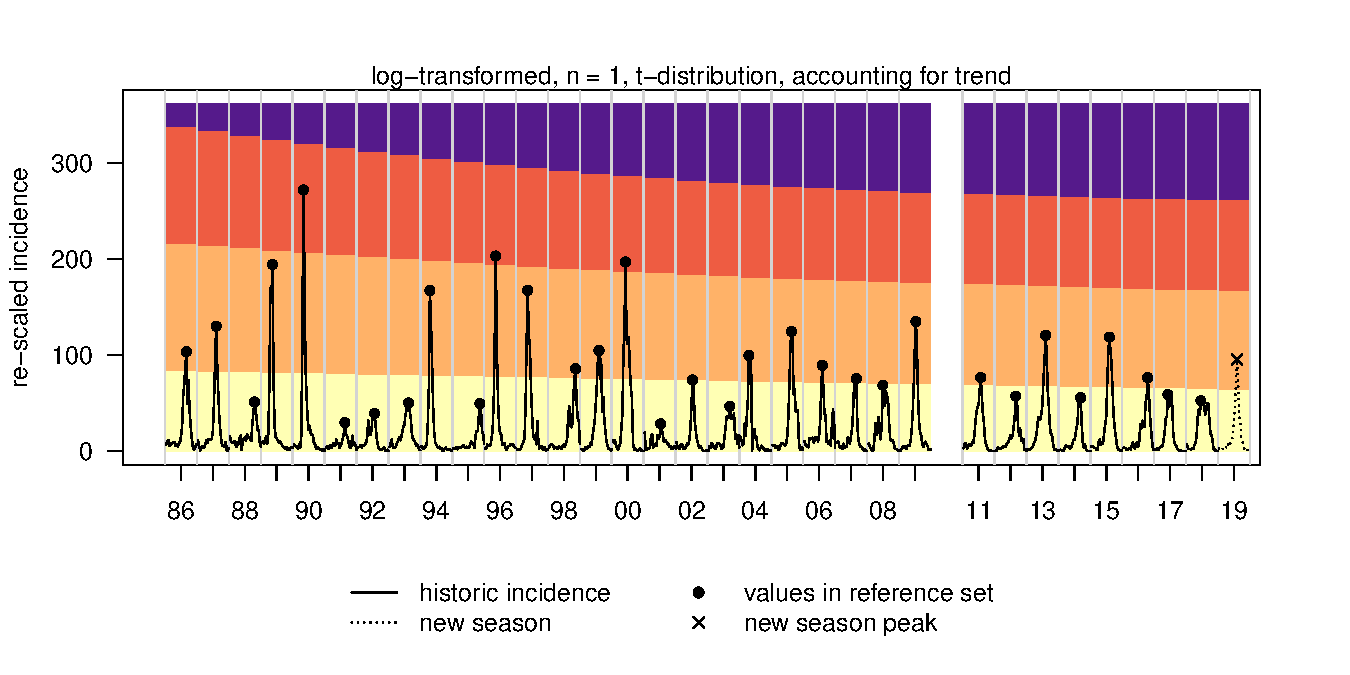
\includegraphics[width = 0.8\textwidth]{figure/illustration_trend.pdf}\vspace{-5mm}
\end{center}
\caption{Illustration of thresholds accounting for a secular trend (using $n = 1$, a log transformation and the $t$-distribution). The data correspond to the years 1986--2019 from the French region of Grand Est, see Section \ref{subsec:data} and Figure \ref{fig:data}. The pandemic season 2009/2010 has been omitted.}
\label{fig:illustration_trend}
\end{figure}



An obvious question is under which conditions thresholds should be corrected for secular trends. In \cite{Farrington1996}, a trend is included if at least three years of weekly data are available and the trend parameter is significant at the 5\% level. This, however, does not seem practical in intensity thresholding, where historical peak values are scarce. The related question of how many observations are needed to reliably fit model \eqref{eq:trend} has been discussed by \cite{Hyndman2007}. However, the authors conclude that this depends on $\beta_1/\sigma_\varepsilon$, meaning that there cannot be any general recommendation. We will return to this question in Section \ref{subsec:results_trends} and the Discussion.

 
\section{Statistical properties}
\label{sec:analytical_results}

In this section we provide some statistical reasoning on the consequences of various implementation choices within the thresholding framework outlined in Section \ref{sec:definitions}. Application-focused readers may find the simulation-based illustration of our findings in Section \ref{sec:simulation} more vivid.

\subsection{Basing thresholds on normal rather than $t$-distributions}
\label{subsec:normal_vs_t}

As discussed in Section \ref{subsec:reformulation} and previously by \cite{Allevius2020}, statistical theory implies that quantiles of a suitable $t$-distribution need be used to obtain valid predictive quantiles for normally distributed outcomes. Using quantiles of a normal distribution as in the original threshold definition \eqref{eq:def_q} will lead to distorted exceedance probabilities unless $m \times n$ is large. Under assumptions (H), (I) and (N), thresholds \eqref{eq:def_q} will be exceeded by a new season peak with probability
$$
1 - F^t_{m\times n - 1}\left[\Phi^{-1}(\alpha)/\sqrt{1 + 1/(m \times n)}\right]
$$
rather than $1 - \alpha$. Here, we denote by $F^t_{m\times n - 1}$ the cumulative distribution function of the $t$-distribution with $m \times n - 1$ degrees of freedom. Figure \ref{fig:calibration_t_normal} displays this relationship for different values of $m \times n$. While for the medium threshold, the exceedance probabilities are slightly too low, the high and very high thresholds are exceeded considerably too often if $m \times n$ is small. For example, if using $m \times n = 10$, the very high threshold is exceeded with probability 5\% rather than 2.5\%. For $m \times n = 5$ this probability increases to 7.4\%. This aspect is most relevant for the WHO method, where the choice $n = 1$ typically leads to small $m \times n$. For $m \times n = 30$ as in the MEM default settings, the differences between the $t$ and the normal distribution are small. However, as will be detailed in the next section, this choice comes with other issues.

\begin{figure}[h!]
\begin{center}
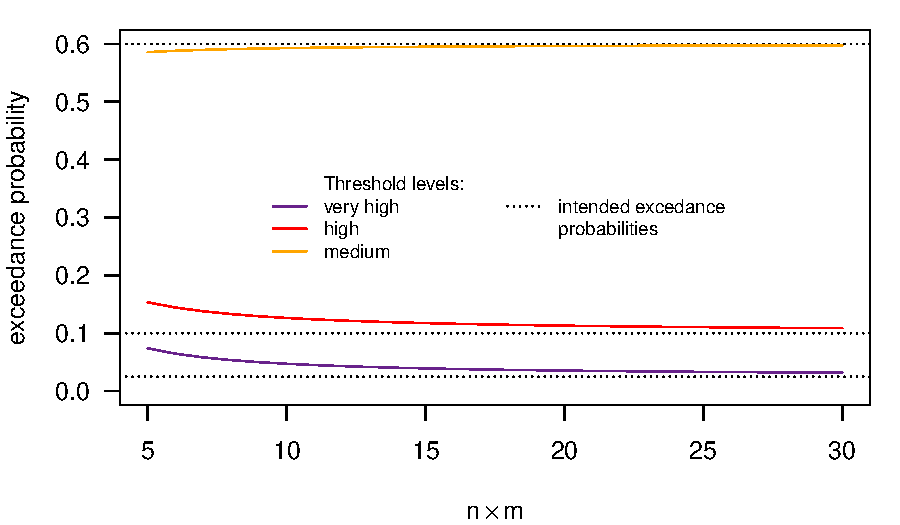
\includegraphics[scale=0.6]{figure/exceedance_prob_normal.pdf}\vspace{-5mm}
\end{center}
\caption{Exceedance probabilities for thresholds \eqref{eq:def_q} based on normal quantiles if assumptions (H), (I), (N) are fulfilled. For medium, high and very high intensity thresholds, exceedance probabilities are displayed as a function of the number $m \times n$ of observations in the reference set. The respective nominal levels are shown as dotted horizontal lines.}
\label{fig:calibration_t_normal}
\end{figure}

\subsection{Choice of the number $n$ of observations used per season}
\label{subsec:choice_n}


We next consider the impact of the number $n$ of observations used per historical season. We assume that no smoothing is applied in Step (a) of the algorithm described in Section \ref{sec:definitions}. Now consider the vectors $\tilde{\mathbf{Y}}_j, j = 1, \dots, m + 1$ from equation \eqref{eq:Y_tilde}. We maintain the assumption that $\tilde{\mathbf{Y}}_1, \dots, \tilde{\mathbf{Y}}_m$ are identically (HB) and independently (IB) distributed. However, we abandon the assumptions that their elements are identically (HW) and independently (IW) distributed, as this is at odds with the fact that $Y_j^{(1)} \geq Y_j^{(2)} \geq Y_j^{(m)}$. We denote the theoretical mean and covariance of $\tilde{\mathbf{Y}}_1, \dots, \tilde{\mathbf{Y}}_m$ by
\begin{align}
\mathbb{E}\left(\tilde{\mathbf{Y}}_j\right) = \boldsymbol{\mu} = \left(\begin{array}{c}
\mu_1\\
\vdots\\
\mu_n
\end{array}\right) \ \ \ \text{and} \ \ \ \text{Cov}\left(\tilde{\mathbf{Y}}_j\right) = \boldsymbol{\Sigma} =
\left(\begin{array}{ccc}
\sigma_{1, 1} & \cdots & \sigma_{1, n}\\
\vdots & \ddots &\vdots\\
\sigma_{n, 1} & \cdots & \sigma_{n, n}
\end{array}\right).
\end{align}
To make notation more intuitive we also write $\sigma^2_i = \sigma_{i, i}$. Remember that thresholds are based on the reference set $\mathcal{Y}$, which pools the elements of $\tilde{\mathbf{Y}}_1, \dots, \tilde{\mathbf{Y}}_m$. It can be shown that the expectations of the empirical mean $\bar{Y}$ and variance $S^2$ of the observations in the reference set are
\begin{align}
\mathbb{E}(\bar{Y}) & = \frac{1}{n} \sum_{i = 1}^n \mu_i,
\label{eq:expectation_mu}\\
\mathbb{E}(S^2) & = \frac{m}{mn - 1} \sum_{i = 1}^n (\sigma_{i}^2 + \mu_i^2) \ - \ \frac{1}{n(mn - 1)} \sum_{i = 1}^n \sum_{i' = 1}^n \sigma_{i,i'} \ - \ \frac{m}{n(mn - 1)}\left(\sum_{i = 1}^n \mu_i\right)^2,
\label{eq:expectation_sigma2}
\end{align}
respectively. Moving to the resulting thresholds, we get
\begin{align}
\mathbb{E}(\hat{q}_{Y, \alpha}) & \approx \mathbb{E}(\bar{Y}) + t_{m\times n - 1, \alpha} \times \left(1 + \frac{1}{m\times n} \right) \times \sqrt{\mathbb{E}(S^2)}
\label{eq:expectation_q}
\end{align}
when using formulation \eqref{eq:q_Y_t}; for the original version \eqref{eq:def_q}, the formula simplifies accordingly. For the thresholds on the original scale
\begin{align}
% \mathbb{E}(\hat{q}_{X, \alpha}) & \approx f^{-1}\left\{\mathbb{E}(\bar{Y}) + t_{m\times n - 1, \alpha} \times \left(1 + \frac{1}{m\times n} \right) \times \sqrt{\mathbb{E}(S^2)}\right\}
\mathbb{E}(\hat{q}_{X, \alpha}) & \approx f^{-1}\left\{\mathbb{E}(\hat{q}_{X, \alpha})\right\}
\label{eq:expectation_q2}
\end{align}
usually holds in good approximation in our setting (i.e., with $f$ the identity function or natural logarithm). Details are provided in Supplement B.3.

For $n = 1$, $\bar{Y}$ and $S^2$ are unbiased estimators of $\mu_1$ and $\sigma^2_1$. Under assumptions (HB), (IB) and (N), it is clear that thresholds based on a suitable $t$-distribution (or, for sufficiently large $m$, normal distribution) will then be exceeded by a new peak $X_{m + 1}^{(1)}$ with the intended probabilities (see Section \ref{subsec:reformulation}). However, for $n > 1$ this will generally not be the case. Equations \eqref{eq:expectation_mu}--\eqref{eq:expectation_q} tell us by how much the expected thresholds change in this case. By the definition of $\mu_i$, $\mathbb{E}(\bar{Y})$ decreases in $n$. While the expected thresholds also depend on $\mathbf{\Sigma}$, this downward bias will usually translate to the $\hat{q}_{Y, \alpha}$. As a consequence, when choosing $n > 1$, one must expect to classify a larger number of season peaks as high or very high intensity. 

Intuitively speaking, including observations which are close to peaks, but not actually peaks, dilutes the reference set and pulls thresholds downward. When choosing $n = 30/m$ as suggested for the MEM, thresholds will tend to increase the larger $m$. Consequently, the probability of exceeding thresholds will decrease, approaching the nominal levels from above. 


\subsection{Smoothing of time series prior to computing thresholds}
\label{subsec:smoothing}

Next we assess the role of smoothing historical data prior to computing thresholds. As derivations get tedious otherwise, we only consider the case where $f$ is the identity function, i.e., no transformation is applied to the reference set and thus $
Y^{(i)}_j = X^{(i)}_j$. Also, as smoothing and multiple observations per season are generally not used in parallel we assume $n = 1$. Now denote by $p_j$ the peak week of the smoothed incidence in season $j$ such that for $l > 1$
\begin{equation}
Y_j^{(1)} =  X_j^{(1)} = X^{\text{smo}}_{j, p_j} = \frac{1}{l} \sum_{d = 0}^{l - 1} X^{\text{raw}}_{j, p_j - d}.\label{eq:Y_1_smoothing}
\end{equation}
Moreover, we define a random vector which contains the observations $X^{\text{raw}}_{j, p_j}, \dots, X^{\text{raw}}_{j, p_j - l + 1}$ (i.e., those averaging to $Y_j^{(1)}$) in decreasing order,
$$
\tilde{\mathbf{X}}^\text{raw}_j = \begin{pmatrix} \tilde{X}_j^{\text{raw}, (1)} & = \ \ \max(X^{\text{raw}}_{j, p_j}, \dots, X^{\text{raw}}_{j, p_j - l + 1}) \\ \vdots & \vdots \\ \tilde{X}_j^{\text{raw}, (l)} & = \ \ \min(X^{\text{raw}}_{j, p_j}, \dots, X^{\text{raw}}_{j, p_j - l + 1}) \end{pmatrix}.
$$
Again we maintain assumptions (HB) and (IB) on the independence and homogeneity between seasons, but relax their within-season counterparts (HW) and (IW). The theoretical mean and covariance matrix of $\tilde{\mathbf{X}}^\text{raw}_j$ are denoted by
\begin{align}
\mathbb{E}\left(\tilde{\mathbf{X}}^\text{raw}_j\right) = \boldsymbol{\mu}^\text{raw} = \left(\begin{array}{c}
\mu^\text{raw}_1\\
\vdots\\
\mu^\text{raw}_l
\end{array}\right) \ \ \ \text{and} \ \ \ \text{Cov}\left(\tilde{\mathbf{X}}^\text{raw}_j\right) = \boldsymbol{\Sigma}^\text{raw} =
\left(\begin{array}{ccc}
\sigma^\text{raw}_{1, 1} & \cdots & \sigma^\text{raw}_{1, l}\\
\vdots & \ddots &\vdots\\
\sigma^\text{raw}_{l, 1} & \cdots & \sigma^\text{raw}_{l, l}
\end{array}\right),
\end{align}
respectively. Note that by construction we have $\mu^\text{raw}_1 \geq \mu^\text{raw}_2 \geq \dots > \mu^\text{raw}_l$. As we assumed $n = 1$, the reference set $\mathcal{Y}$ consists simply of $Y^{(1)}_1, \dots, Y^{(1)}_m$ as given in equation \eqref{eq:Y_1_smoothing}. It is straightforward to show that in this case the expectations of $\bar{Y}$ and $S^2$ are
\begin{align}
\mathbb{E}(\bar{Y}) = \frac{1}{l} \sum_{i = 1}^l \mu^\text{raw}_i, \ \ \ 
\mathbb{E}(S^2) = \frac{1}{l^2} \sum_{i = 1}^l \sum_{i' = 1}^l \sigma^\text{raw}_{i', i}.
\label{eq:expectation_moments_smoothing}
\end{align}
These can be plugged into equation \eqref{eq:expectation_q} to approximate the expected thresholds. 

The expressions from \eqref{eq:expectation_moments_smoothing} are obviously unbiased estimators of the mean and variance of smoothed peak values  $Y_j^{(1)} =  X_j^{(1)} = X^{\text{smo}}_{j, p_j}$. Now assume that normality (N) holds and that thresholds are applied to $Y_{m + 1}^{(1)}$, i.e., a smoothed new peak value. The thresholds based on a $t$-distribution (or, for sufficiently large $m$, a normal distribution) will then have the desired exceedance probabilities. This, however, is not the case if thresholds are applied to unsmoothed new peak values, as done in the WHO method. For $l > 1$, unsmoothed peaks by construction exceed smoothed peaks, and will thus also exceed thresholds more frequently. To ensure calibration of thresholds, it is thus necessary to either smooth historical \textit{and} new peaks, or neither of the two.



\subsection{Sensitivity and specificity under normality and $n = 1$}
\label{subsec:theory_sensitivity}

While in the previous sections we focused on calibration and expected thresholds, we now turn to the resulting sensitivity and specificity. As discussed in Section \ref{subsec:choice_n}, the assumptions (HW) and (IW) on within-season homogeneity and independence are implausible if $n > 1$. We therefore focus again on the case where $n = 1$ observation is used per historical season and thus $\mathcal{Y} = \{Y_1^{(1)}, Y_2^{(1)}, \dots, Y_m^{(1)}\}$. For the following we require assumptions (HB), (IB) and (N), which in this case amount to
\begin{equation}
Y_1^{(1)}, \dots, Y_m^{(1)}, Y_{m + 1}^{(1)} \stackrel{\text{i.i.d.}}{\sim} \text{N}(\mu_1, \sigma^2_1).
\end{equation}
Defining the threshold $\hat{q}_{Y, \alpha}$ via quantiles of the normal distribution as in \eqref{eq:def_q}, it can be shown that
\begin{equation}
\hat{q}_{Y, \alpha} \stackrel{\text{approx}}{\sim} \text{N}\left\{\mu_1 + z_\alpha \sigma_1,\ \ \sigma_1^2 \times \left(\frac{1}{m} + \frac{z_\alpha^2}{2(m - 1)} \right) \right\}.
\label{eq:q_Y}
\end{equation}
For definition \eqref{eq:q_Y_t} based on the $t$-distribution a slightly more involved expression is given in Supplement B.5. Based on this we can approximate the sensitivity and specificity of our thresholding procedure at level $\alpha$. The sensitivity is the probability that given the new transformed peak $Y_{m + 1}^{(1)}$ is truly among the $(1 - \alpha) \times 100\%$ highest peaks with respect to an underlying stationary distribution,
$$
Y_{m + 1}^{(1)} \geq q_{Y, \alpha} = \mu_1 + z_\alpha \sigma_1,
$$
it will also be classified as such, i.e.,
$$
Y_{m + 1}^{(1)} \geq \hat{q}_{Y, \alpha}.
$$
It can be shown that the probability in question can be approximated by
\begin{equation}
\text{sens}_\alpha = \text{Pr}\left(Y_{m + 1}^{(1)} > \hat{q}_{Y, \alpha} \ \mid \ Y_{m + 1}^{(1)} > q_{Y, \alpha}\right) \approx \int_{z_\alpha}^\infty \phi(y) \times \Phi\left(\frac{y - z_\alpha}{\sqrt{\frac{1}{m} + \frac{z_\alpha^2}{2(m - 1)}}}\right) \text{d}y.
\label{eq:sens}
\end{equation}
Here, $\phi$ and $\Phi$ are the density function and cumulative distribution function of the standard normal distribution, while $z_\alpha$ is its $\alpha$ quantile. We note that this expression depends on $\alpha$ and $m$, but not $\mu_1$ and $\sigma^2_1$. Similarly, the specificity can be approximated by
\begin{equation}
\text{spec}_\alpha = \text{Pr}\left(Y_{m + 1}^{(1)} < \hat{q}_\alpha \ \mid \ Y_{m + 1}^{(1)} < q_{Y, \alpha}\right) \approx \int_{-\infty}^{z_\alpha}\phi(y) \times \left\{1 - \Phi\left(\frac{y - z_\alpha}{\sqrt{\frac{1}{m} + \frac{z_\alpha^2}{2(m - 1)}}}\right)\right\} \text{d}y.
\label{eq:spec}
\end{equation}
The positive predictive value can be computed using the formula \citep{Altman1994}
\begin{equation}
\text{PPV}_\alpha = \text{Pr}(Y_{m + 1}^{(1)} > q_{Y, \alpha} \ \mid Y_{m + 1}^{(1)} > \hat{q}_\alpha) = \frac{(1 - \alpha) \times \text{sens}_\alpha}{(1 - \alpha) \times \text{sens}_\alpha + \alpha \times (1 - \text{spec}_\alpha)}.
\label{eq:ppv}
\end{equation}
Expressions \eqref{eq:sens}--\eqref{eq:ppv} have no simpler closed form, but they are straightforward to evaluate numerically. Again, slightly more involved versions of these formulas can be obtained for thresholds based on the $t$-distribution. These are provided in Supplement B.5, along with the derivations.

In Figure \ref{fig:sens_spec_ana} we visualize the sensitivity, specificity and positive predictive values as a function of $m$ and $\alpha = 0.4, 0.9, 0.975 $. As the theoretical approximations may not be very accurate for small $m$, we also show simulation-based versions. For the high and very high thresholds, the $t$-distribution leads to lower sensitivity, but higher specificity and PPV than the normal distribution (which is a consequence of the $t$-distribution being more dispersed). Little surprisingly, the sensitivity, specificity and positive predictive values increase in $m$. The sensitivity and PPV are lowest for the very high threshold at $\alpha = 0.975$. For the most practically relevant values of $5 \leq m \leq 10$, the PPV is only between 0.25 and 0.5 in this case. More than half of the seasons flagged as very high intensity will thus be false positives, i.e., peaks which are not actually among the highest 2.5\%. For the high threshold ($\alpha = 0.9$), the respective PPVs are between 0.5 and 0.7.

Even if assumptions (H), (I) and (N) are fulfilled, there are thus natural limits to the classification performance, which for small $m$ and high $\alpha$ are at modest levels. We note that this result is the same irrespective of whether any smoothing has been applied (as long as both historical and new peaks are smoothed). While smoothing will make thresholds less variable, any effect on sensitivity and specificity is canceled out by the fact that smoothed new peaks are likewise less variable.

\begin{figure}[h!]
\begin{center}
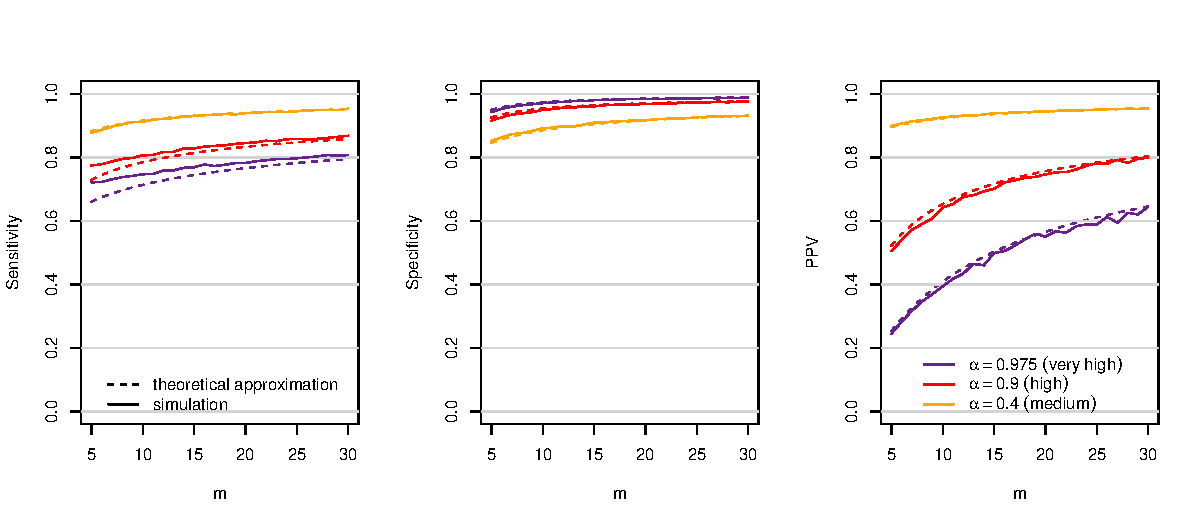
\includegraphics[scale=0.75]{figure/analytical_sens_spec.pdf} \vspace{-5mm}

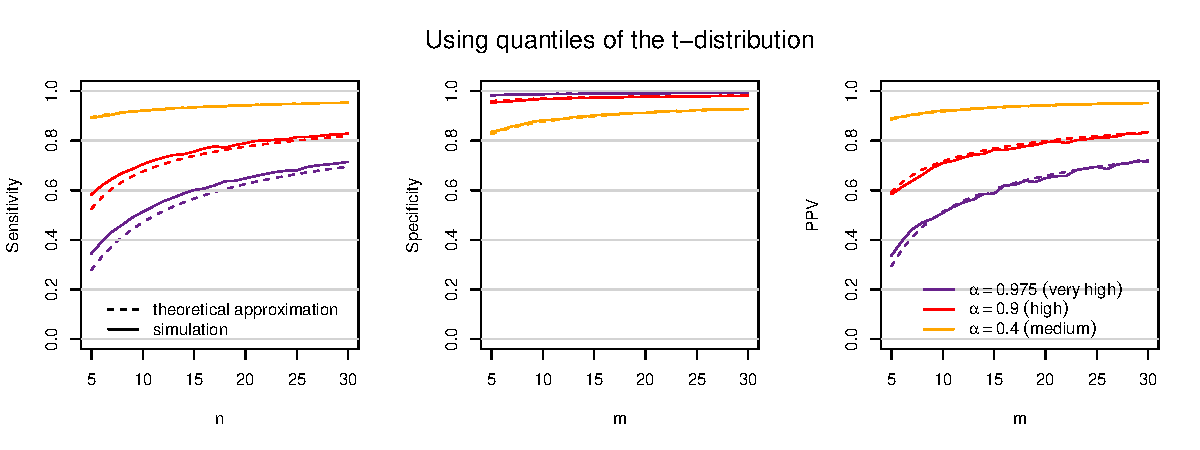
\includegraphics[scale=0.75]{figure/analytical_sens_spec_t.pdf}
\end{center}

\vspace{-10mm}

\caption{Sensitivity, specificity and PPVs with $n = 1$ and under the normality assumption (N), by number $m$ of historical seasons used. Top row: when using the original formulation \eqref{eq:def_q} based on the normal distribution. Bottom: when using formulation \eqref{eq:q_Y_t} based on the $t$-distribution. Dashed lines show the approximations \eqref{eq:sens}--\eqref{eq:ppv}, solid lines simulation results.}
\label{fig:sens_spec_ana}
\end{figure}



\subsection{Basing thresholds on confidence intervals}
\label{subsec:cis}

The thresholds from equation \eqref{eq:def_q} have previously been referred to as upper ends of one-sided confidence intervals for the arithmetic or geometric mean of the reference observations \citep{WHO2014, Vega2015}. As mentioned in Section \ref{subsec:reformulation}, this is imprecise terminology and the thresholds should instead be interpreted as predictive quantiles. The use of actual confidence interval limits, however, is also possible in the \texttt{mem} package (see Supplement B.1). Equation \eqref{eq:expectation_q} then becomes
$$
\mathbb{E}(q_{Y, \alpha}) \approx \mathbb{E}(\bar{Y}) + \frac{z_\alpha}{\sqrt{nm}} \sqrt{\mathbb{E}(S^2)}.
$$
This is not desirable as for increasing $m \times n$ thresholds for all levels $\alpha$ will converge to $\mathbb{E}(\bar{Y})$. Each new season peak will then be classified either as low or as very high intensity. This issue applies to all types of confidence intervals implemented in the package, including those based on boostrapping.

\section{Simulation study}
\label{sec:simulation}

\subsection{Setup}
\label{subsec:simulation_setup}

The analytical results from the previous section involve some approximations and various assumptions on the observations in the reference set $\mathcal{Y}$. In the following we study the respective aspects empirically in a simulation study. To realistically mimic the seasonal patterns of influenza, we re-sample historical surveillance data rather than generating fully synthetic data. This enables us to assess the behaviour of thresholds if assumptions (HW), (IW) and (N) are violated in a realistic manner. We note that assumptions (HB) and (IB) hold by construction of the simulation scheme, i.e., we will not be able to assess how violations of these assumptions affect thresholds. For the re-sampling scheme, assume $M$ seasons of historical data on a measure of influenza activity are available. We then repeat the following steps 500 times:

\begin{itemize}
\item[(a)] Sample a sequence of 15 seasons from the $M$ available seasons. This is done with equal probability for each season and \textit{with replacement}, meaning that the same season can appear more than once. This approach is called the \textit{seasonal block bootstrap} \citep{Politis2001}.
\item[(b)] For each value $m = 5, \dots, 15$:
\begin{itemize}
\item[(i)] Restrict the generated sequence to the first $m$ seasons.
\item[(ii)] Compute thresholds for medium, high and very high intensity ($\alpha = 0.4, 0.9, 0.975$). This is done using a number of variations of the thresholding procedure, see below.
\item[(iii)] Evaluate which of the $M$ historical season peaks would be classified as low, moderate, high and very high.
\end{itemize}
\item[(c)] Compute summary statistics including mean thresholds, exceedance probabilities, sensitivities, specificities and PPVs. Following the reasoning from Section \ref{sec:desirable_properties}, the true intensity levels of the different seasons are determined based on the empirical distribution of all $M$ seasons (i.e., the 2.5\% highest peaks are very high intensity, the following 7.5\% high intensity etc.).
\end{itemize}
The range $m =5, \dots, 15$ is motivated by the values found in real-world applications, see Section \ref{sec:review}. We compute thresholds using nine variations of the approach described in Section \ref{sec:definitions}. In a first step, we assess the MEM and WHO method in their current form \eqref{eq:def_q}, i.e. based on quantiles of the normal distribution. Specifically, the following settings are considered:
\begin{enumerate}
\item[(a)] no smoothing, no transformation of the reference set, $n = 1$. This corresponds to the WHO method, but without the optional smoothing step.
\item[(b)] no smoothing, logarithmic transformation of the reference set, $n = 1$.
\item[(c)] same as (a), but using $n = 30/m$.
\item[(d)] same as (b), but using $n = 30/m$. This corresponds to the default MEM approach.
\end{enumerate}
\noindent To study the impact of smoothing we apply the following settings:
\begin{enumerate}
\item[(e)] smoothing with $l = 3$ (alternatively $l = 7$), log transformation of the reference set, $n = 1$, thresholds applied to unsmoothed new peaks. This corresponds to the WHO method with the optional log transformation applied.
\item[(f)] same as (e), but thresholds applied to smoothed new peaks.
\end{enumerate}
We then address the two extensions of the thresholding procedure proposed in Section \ref{sec:formalization_extension}.
\begin{enumerate}
\item[(g)] no smoothing, logarithmic transformation of the reference set, $n = 1$, using quantiles of a $t$ rather than normal distribution. Thresholds are thus based on equation \eqref{eq:q_Y_t} rather than \eqref{eq:def_q}.
\item[(h)] same as (g), but accounting for a secular trend using equation \eqref{eq:trend}. To assess this setting, a secular trend is artificially added to the re-sampled time series, see Section \ref{subsec:results_trends}.
\end{enumerate}
Finally, we illustrate the behaviour if confidence rather than prediction intervals are used.
\begin{enumerate}
\item[(i)] no smoothing, log transformation of the reference set, $n = 1$ (alternatively $n = 30/m$), using confidence rather than prediction intervals.
\end{enumerate}
All analyses were performed using the R language for statistical computing \citep{RCT2020} and the package \texttt{mem} \citep{Lozano2020}. For points (g) and (h), the method was re-implemented independently (though as noted previously, setting (g) has in the meantime been added to the development version of \texttt{mem}).

\subsection{Data}
\label{subsec:data}

We use publicly available data on the estimated weekly incidence of influenza-like illness per 100,000 inhabitants in France, 1986--2019, published by Réseau Sentinelles (INSERM/Sorbonne Université, \url{https://www.sentiweb.fr}, \citealt{Flahault2006}). These are available at the national and regional levels. To make statements about the ``very high'' category, we require a larger set of historical data than the available 34 seasons. We therefore pool curves from the 12 continental French administrative regions. As the overall level of ILI incidence varies considerably across regions, we scale all data such that the average season peak per region is 100. As the incidence curves from the Corse island region differ substantially from the other regions we exclude them. Moreover, the pandemic 2009/2010 season was removed. In total we then dispose of $12 \times 33 = 396$ season curves.

Figure \ref{fig:data} shows an illustration of the re-scaled data from two regions (Grand Est and Nouvelle Aquitaine), along with descriptive plots. In the bottom left we show boxplots of the first through sixth largest observation per season. Not surprisingly, values on average get smaller for increasing ranks. They also get less dispersed, meaning that variability among e.g.\ the sixth largest observations per season is smaller than among peak values. Values from the same season are strongly correlated across ranks. The next panel shows the distribution of peaks without smoothing ($l = 1$) and with smoothing windows of $l = 3$ and $l = 7$. As expected, peak values get lower and less dispersed when smoothing is applied. The remaining panels show normal QQ plots of untransformed and log-transformed peak values. After transformation the distribution is roughly normal.

To assess the sensitivity of our results to the choice of data set we re-run all simulations using  weekly weighted ILI (wILI) data from the US. These stem from the from CDC \textit{FluView} project (Charbonneau and James, 2019), cover the years 1998–2018, and were
obtained via the CDC \textit{FluSight} influenza forecasting platform (\url{https://github.com/FluSightNetwork/cdc-flusight-ensemble/}). Reported values correspond to the fraction of general practitioner visits which are due to influenza-like symptoms. To increase the number of available seasons we again pool national-level data and data from the ten Health and Human Services (HHS) regions, re-scaling data to mean peak values of 100. In total we thus obtain $11 \times 19 = 209$ historical seasons. Results based on the US data have been moved to Supplement D and are briefly discussed in Section \ref{subsec:results_us}.

\begin{figure}[h]
\center
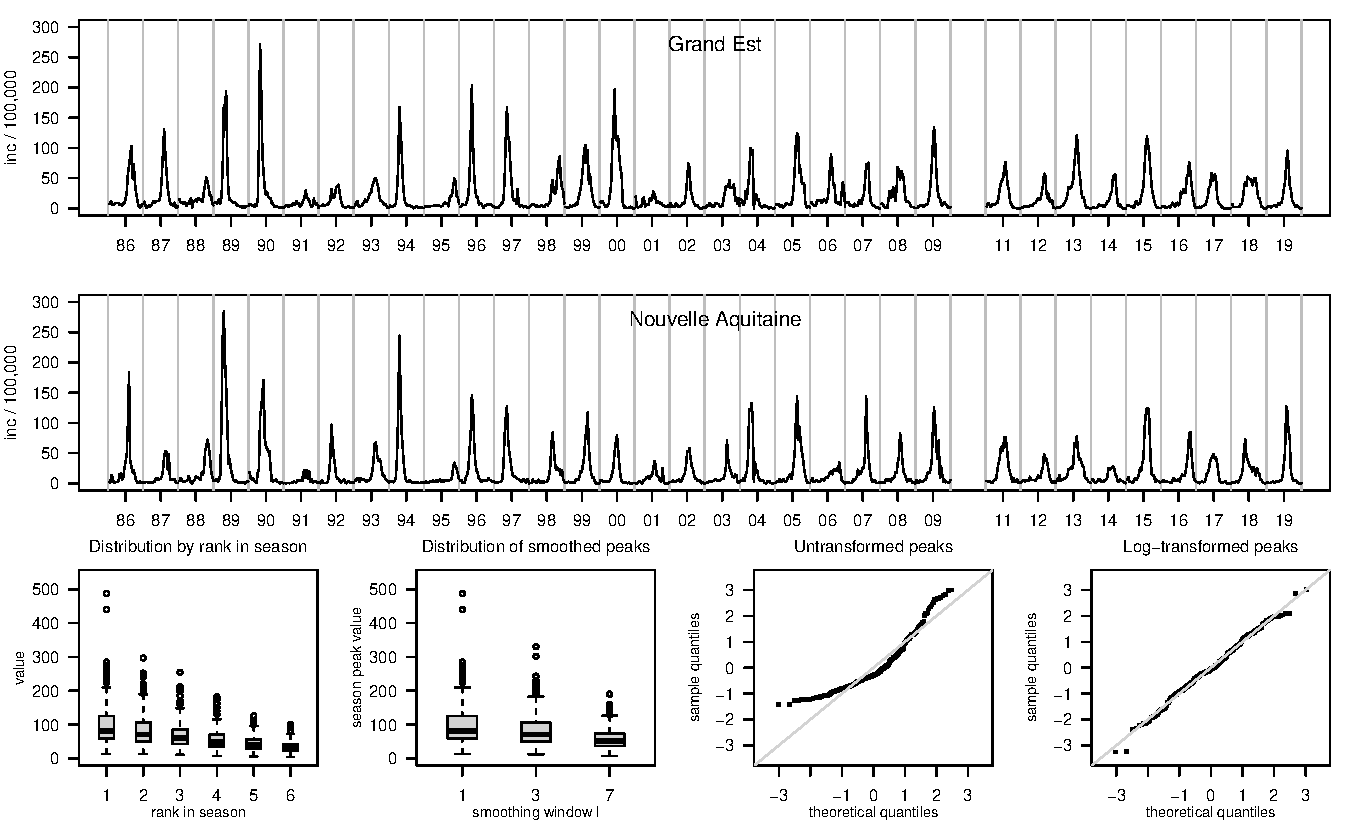
\includegraphics[width=0.9\textwidth]{figure/plot_data_fr.pdf}
\caption{Top and middle row: Re-scaled estimated numbers of weekly ILI cases in the French regions of Grand Est and Nouvelle Aquitaine, 1985--2019, with the pandemic season 2009/2010 removed. Off-season weeks are omitted, with grey lines delimiting the different seasons. The bottom row shows descriptive plots of the distribution of season peaks. First: Boxplots of incidence values by rank within season. Second: Boxplot of smoothed peak values as a function of the smoothing window width $l$. In these two plots, light grey lines link values stemming from the same season. The numbers above the boxplots indicate the Pearson correlation between the values shown in the first boxplot ($i = 1$ or $l = 1$, respectively) and the boxplot in question. Third: Normal QQ plot of untransformed peak values. Fourth: Normal QQ plot of log-transformed peak values.}
\label{fig:data}
\end{figure}

\subsection{Results based on French data}

\subsubsection{Choice of transformation $f$ and number $n$ of observations used per season}
\label{subsubsec:n}

\textbf{Thresholds and threshold exceedance.} Figure \ref{fig:results1} summarizes thresholds resulting from different combinations of transformation function $f$ and number $n$ of observations used per season (specifications a--d from Section \ref{subsec:simulation_setup}). Here, all thresholds are based on a normal distribution as in \eqref{eq:def_q}. For each case we show mean thresholds, along with the empirical 5\% and 95\% quantiles, and the shares of new seasons classified into the different categories. This is complemented with summaries of the sensitivity, specificity and positive predictive value. All results are shown as a function of the number $m$ of historical seasons used. Where applicable, the simulation results displayed as squares are complemented by analytical approximations shown as lines. These have been computed using equations \eqref{eq:expectation_q2} and \eqref{eq:sens}--\eqref{eq:ppv} with empirical means and covariances plugged in.

\begin{figure}[h!]
\centering
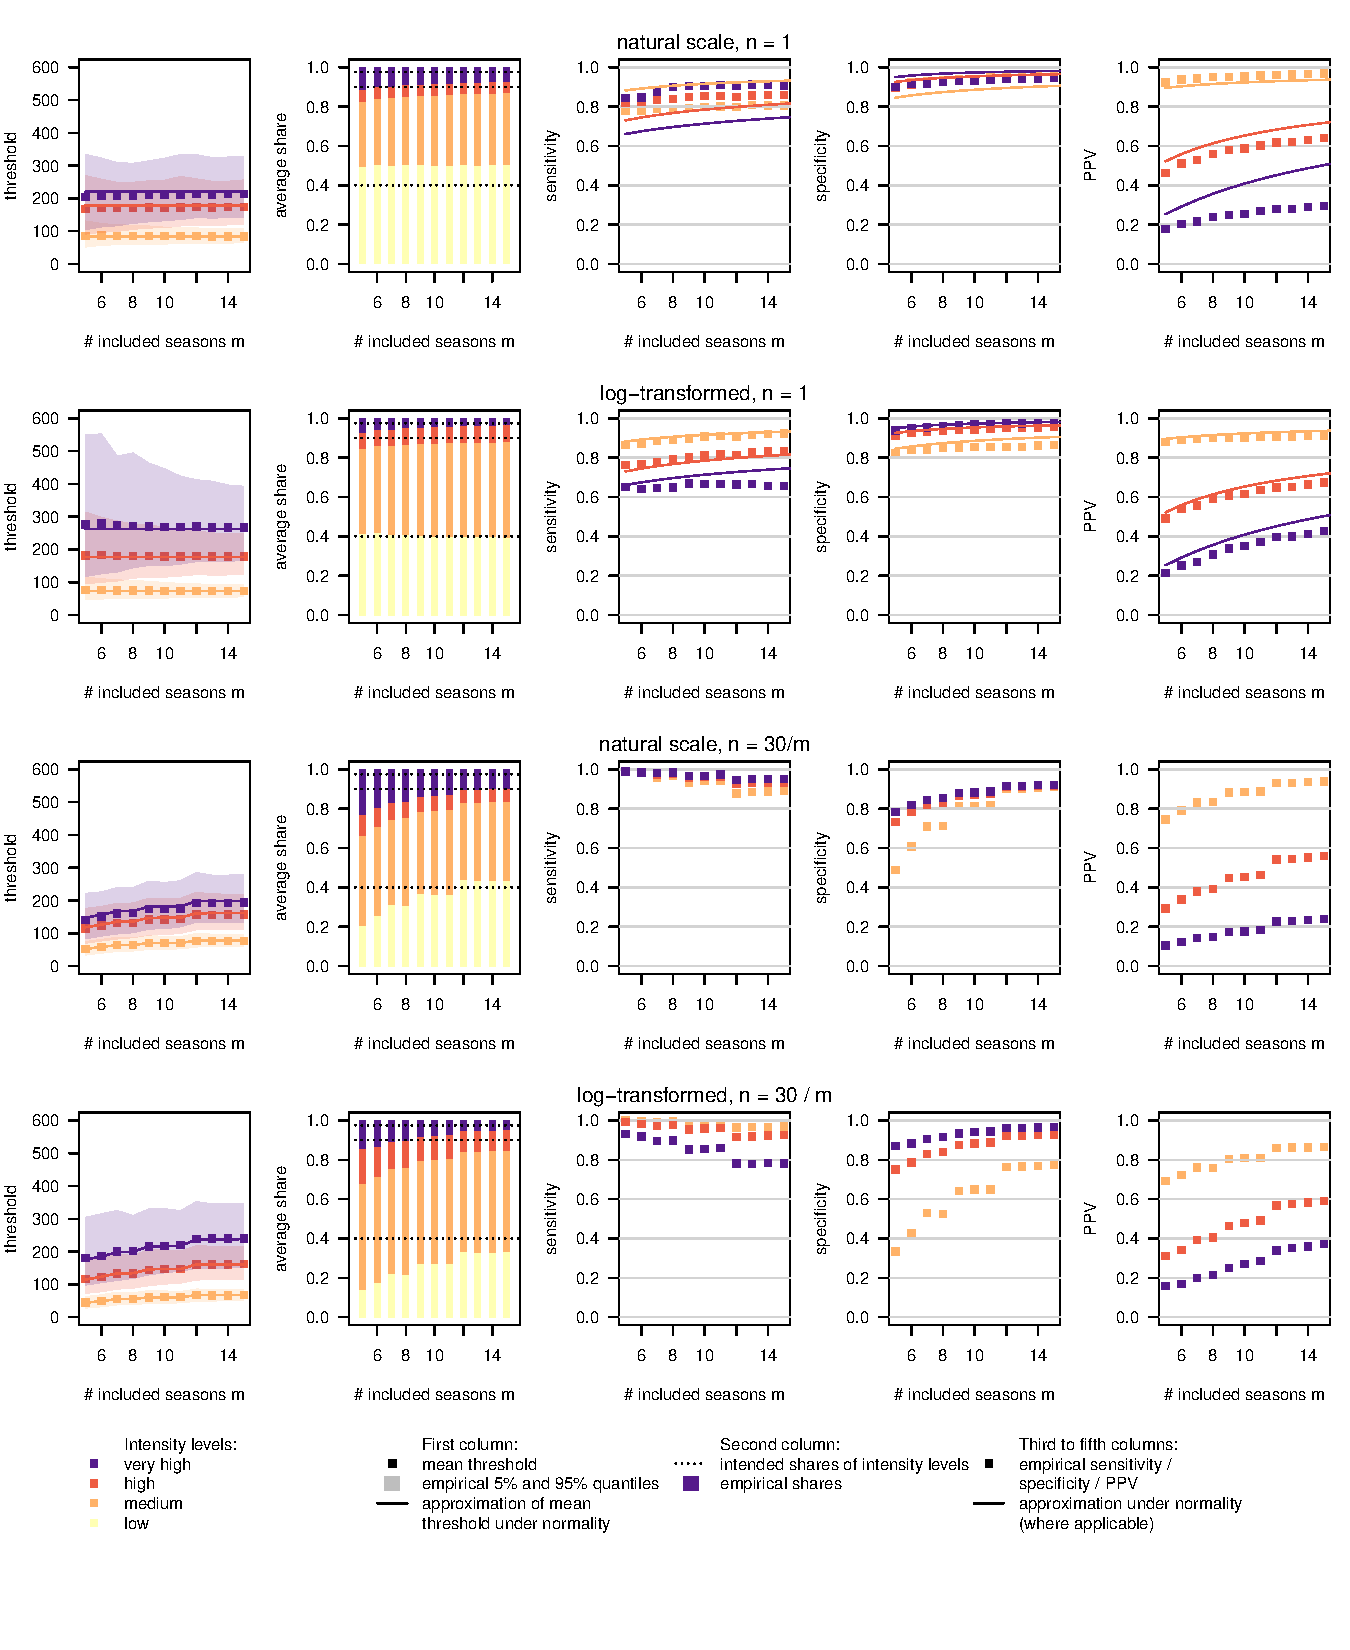
\includegraphics[width=0.9\textwidth]{figure/plot_fr.pdf}

\vspace{-1.5cm}

\caption{Impact of the choice of $n$ and transformation function $f$. First column: simulation-based average intensity thresholds (squares) along with bands delimited by the empirical 5\% and 95\% quantiles. Analytical approximations of mean threshold values (computed from empirical means and covariances) are displayed as lines. Second column: resulting average shares of season peaks classified as low, medium, high and very high intensity. Third to fifth columns: sensitivity, specificity and PPVs of the different thresholds. Simulation results are shown as squares. Where available analytical approximations are shown as lines.}
\label{fig:results1}
\end{figure}

Thresholds for high and very high intensity are higher when a log transformation is employed. This leads to better calibration, i.e., the shares of seasons exceeding the high or very high thresholds are closer to the intended levels of 10\% and 2.5\%. Indeed, when using $n = 1$ observation per season and $m \geq 10$ historical seasons, the thresholds based on log-transformed data have close to nominal exceedance rates. Without this transformation, new season peaks are classified as very high in roughly 10\% rather than 2.5\% of the cases. This indicates that the normal assumption is more appropriate after log tansformation, as already visible from the normal QQ plots in Figure \ref{fig:data}.

As implied by the reasoning from Section \ref{subsec:choice_n}, letting the number of observations used per season depend on the number of available seasons via $n = 30/m$ leads to average thresholds which increase in $m$. When using a log transformation, they increase from 180 for $m = 5, n = 6$ to 218 for $m = 10, n = 3$ and 240 for $m = 15, n = 2$. If we choose $n = 1$ irrespective of $m$, as recommended in Section \ref{subsec:choice_n}, the average is around 270. Including historical observations which are not actual peaks thus leads to a considerable lowering of thresholds and increases the number of alerts for high and very high influenza activity. For $m = 5, n = 6$ the proportion of season peaks classified as very high is 15\% if a log transformation is used and 24\% otherwise. As can be seen from the fourth column, this is due to poor specificity, and as shown in the fifth column, leads to low positive predictive values. In the most extreme case where $m = 5$ seasons are used without a transformation, only one in ten seasons peaks classified as very high is actually from the 2.5\% most extreme peaks. We note, however, that even the most well-behaved specification with $n = 1$ and a log transformation only yields a PPV slightly above 20\% for $m = 5$. For $m = 15$ this value roughly doubles. Our theoretical approximation is well aligned with the simulation results here (but much less so if no log transformation is used, as in this case the normality assumption is poorly fulfilled).


It can be noted that the thresholds generally have high variability (see the shaded bands in the first column of Figure \ref{fig:results1}). This is particularly pronounced for the very high threshold, and even more so if a logarithmic transformation is used. This reflects the general difficulty of estimating extreme quantiles from a small number of observations.

\textbf{Confusion matrices.} To complement these results and provide some more intuition on the intensity classifications, Figure \ref{fig:mosaic} shows confusion matrices for thresholds computed with a log transformation and different values of $m$. This represents a more detailed breakup of the results from the second column of Figure \ref{fig:results1}. Note that the perspective differs somewhat from the computation of sensitivities and specificities. There, we focused on \textit{threshold exceedance}, considering for instance whether the medium threshold was exceeded by a peak which was truly at least medium intensity. For the sensitivity of the medium threshold we thus ignored whether a peak which was truly medium intensity also exceeded the high threshold (which was in turn reflected in the specificity of the high threshold). Now we consider not just threshold exceedance, but the exact categorization. This is shown stratified by the true category of a peak, determined via the empirical distribution of all 396 available peaks. %  (the highest 2.5\% are considered very high, the next 7.5\% high, the next 50\% medium and the remaining 40\% low).

For $n = 1$ (top two rows) it can be seen that in all categories misclassifications occur, but become less frequent for larger $m$. The log transformation leads to better classification of truly medium and high peaks, while for truly low or very high peaks results are better without a transformation. This essentially reflects that thresholds are more spaced out when using a log transformation (see Figure \ref{fig:results1}), giving medium and high peaks a better chance of correct classification. The rather modest positive predictive values from Figure \ref{fig:results1} are here reflected by the fact that in most panels, a large part of the peaks classified as very high (purple rectangles) are actually high or medium.

For $n = 30/m$, the miscalibration issues identified previously are again visible. For $m = 5$ and with a log transformation, more than 60\% of truly low peaks are classified as medium; roughly 40\% of medium peaks are classified as high or very high; and close to 75\% of high peaks are classified as very high. As implied by theory, the problem is diminished with increasing $m$.

A natural obstacle to high classification accuracy is that e.g., the highest peaks from the medium category are similar to the lowest ones from the high category. We illustrate this in Supplementary Figure 1, which is a fine-grained version of Figure \ref{fig:mosaic}. Here we display the classification proportions as a function of the true quantile level a season peak corresponds to. These proportions change smoothly, and the chance of misclassification is particularly high for peaks close to the 40th, 90th and 97.5th percentiles of the underlying distribution.

\begin{figure}
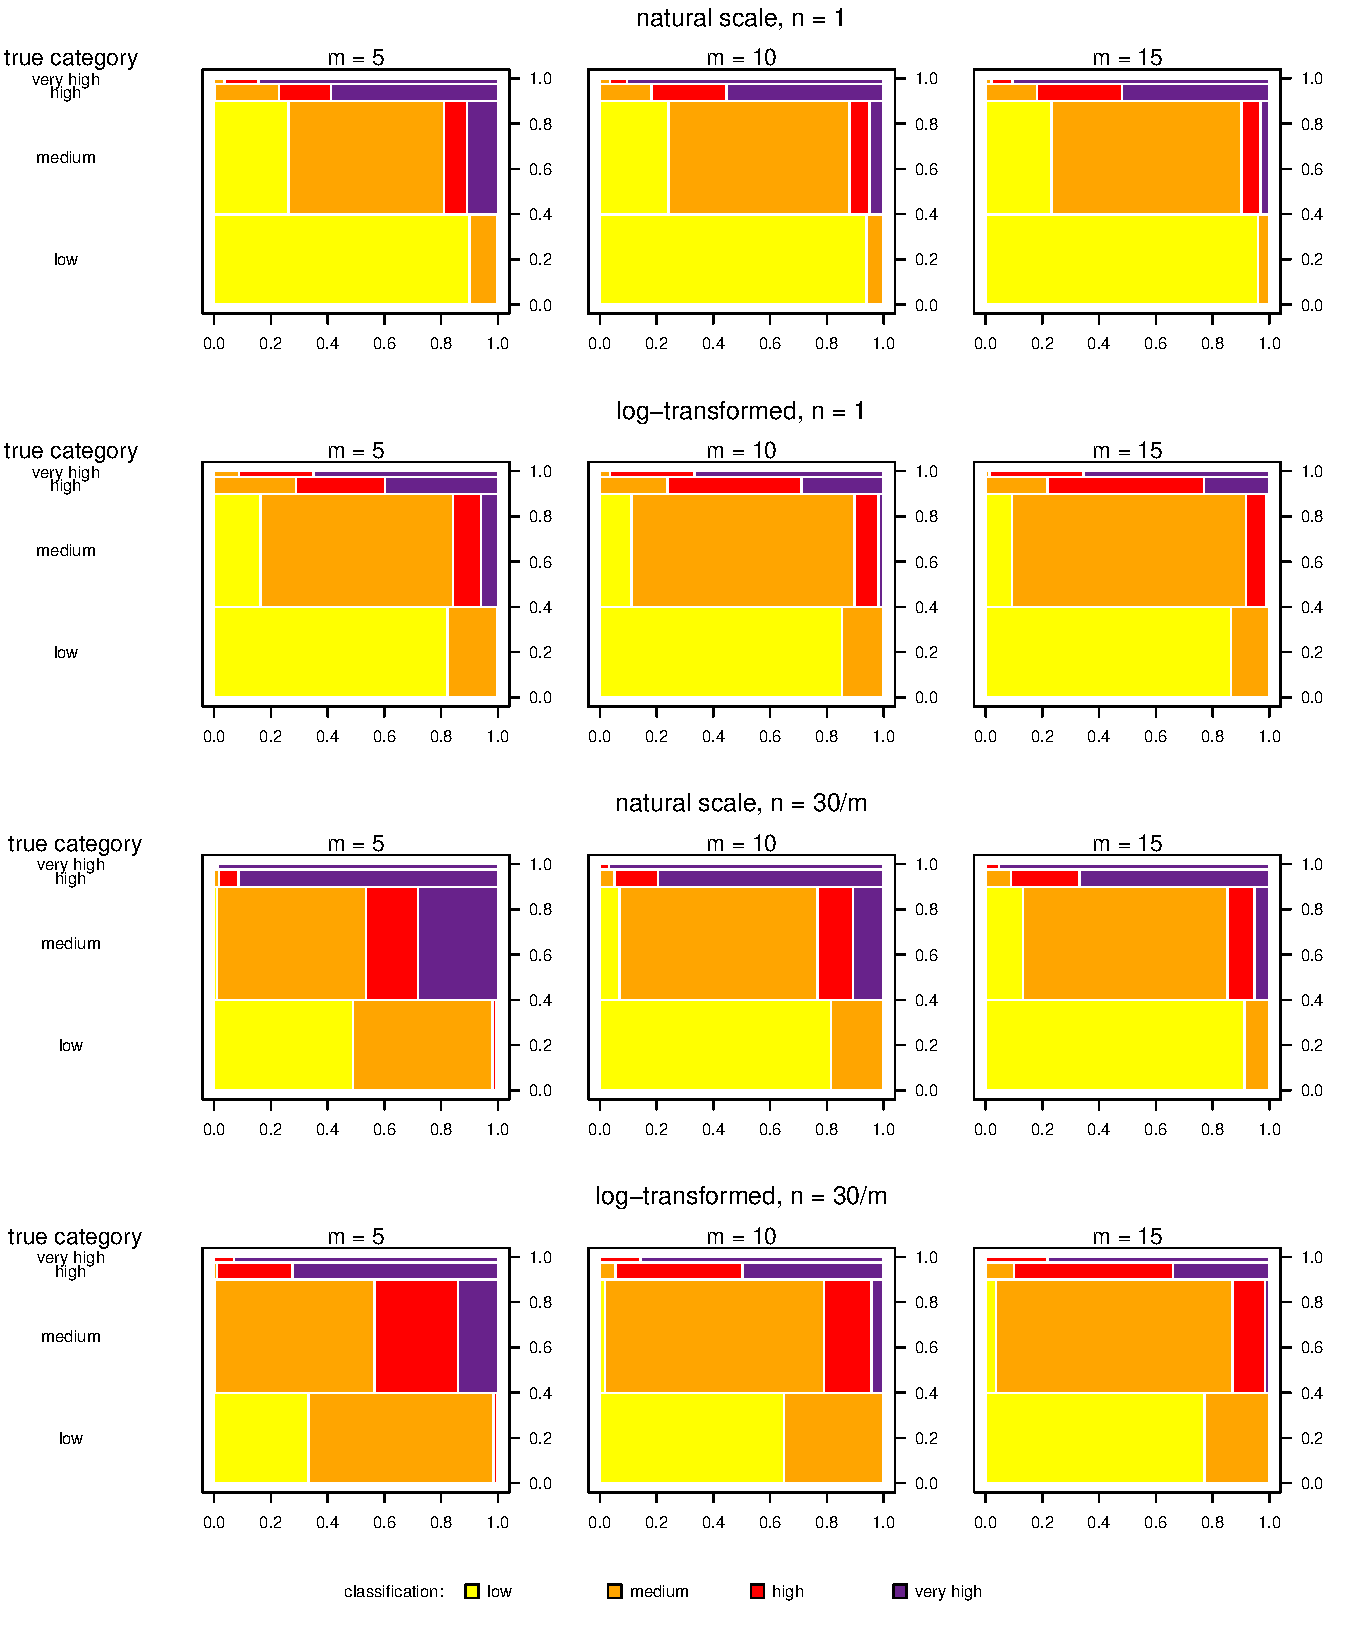
\includegraphics[width=0.9\textwidth]{figure/mosaic_fr.pdf}
\caption{Confusion matrices for intensity classifications obtained with different choices of $n$ and transformation function $f$. Mosaic plots show which fractions of season peaks which are truly very high, high, medium or low are classified into the four categories. The true class is determined with respect to the empirical quantiles of the distribution of peaks: very high (highest 2.5\% of all peaks), high (next 7.5\%), medium (next 50\%), low (lowest 40\% of all peaks).}
\label{fig:mosaic}
\end{figure}



\subsubsection{Smoothing of time series prior to computing thresholds}
\label{subsec:sim_smoothing}

\textbf{Thresholds and threshold exceedance.} We next assess the impact of smoothing historical data prior to computing thresholds (cases e--f from Section \ref{subsec:simulation_setup}). Results for a window size of $l = 3$ and including a log transformation are shown in Figure \ref{fig:results_smoothing}. The top row shows the case where thresholds are applied to unsmoothed new peaks. In accordance with the arguments from Section \ref{subsec:smoothing}, the high and very high thresholds are exceeded more frequently than intended (e.g., almost one in ten seasons classified as very high intensity for $m = 10$). When applying thresholds to smoothed new peaks, the empirical and nominal exceedance levels are better aligned. Thresholds are less variable than without smoothing, but as predicted by theory, sensitivity, specificity and positive predictive values remain similar (compare the second rows of Figures \ref{fig:results1} and \ref{fig:results_smoothing}). We provide a display for a stronger smoothing with $l = 7$ in Supplementary Figure S2. If the resulting thresholds are applied to unsmoothed new peaks, more than a fifth of them is classified as very high.

\begin{figure}[h!]
\centering
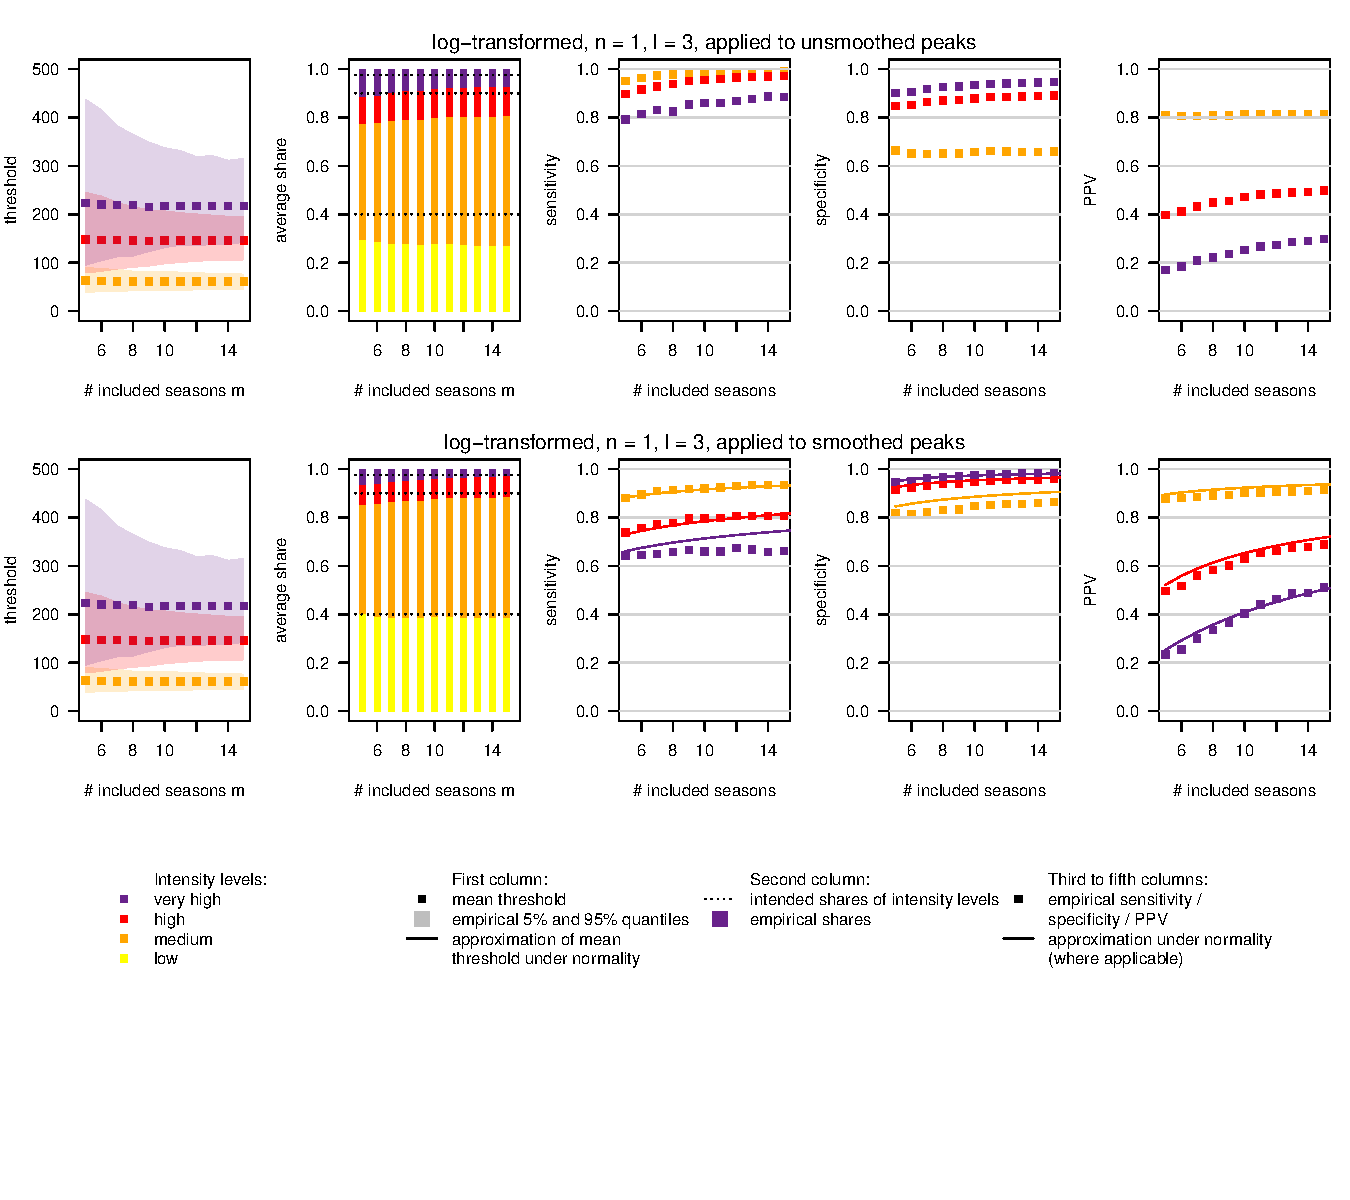
\includegraphics[width=0.9\textwidth]{figure/plot_smoothing3_fr_small.pdf}

\caption{Impact of smoothing of historical data. We applied a moving average with $l = 3$ to the historical time series prior to computing thresholds and subsequently applied them to unsmoothed (top) and smoothed (bottom) new peaks. Results are shown for thresholds computed with a log transformation. See Figure \ref{fig:results1} for details on the plot elements.}
\label{fig:results_smoothing}
\end{figure}


\textbf{Confusion matrices.} We complement this again with confusion matrices in Supplementary Figure S3. When unsmoothed new peaks are classified based on thresholds computed with smoothing, peaks tend to be assigned to too high categories. When thresholds are applied to smoothed new peaks, the results resemble those obtained without smoothing of either historical or new peaks.


\subsubsection{Employing the $t$-distribution}

\textbf{Thresholds and threshold exceedance.} In Figures \ref{fig:results1} and \ref{fig:results_smoothing}, it is evident that even when using $n = 1$, the thresholds are miscalibrated for small $m$. As argued in Sections \ref{subsec:reformulation} and \ref{subsec:normal_vs_t}, in this case it is necessary to base thresholds on a $t$ rather than a normal distribution. Indeed, as visible in Figure \ref{fig:t}, this modification leads to close-to-nominal exceedance fractions across all considered values of $m$ when employing a log transformation. Thresholds computed on the natural scale remain somewhat miscalibrated. A characteristic of these thresholds which may seem surprising is that the average values of the very high and high thresholds decrease in $m$. This is due to the fact that well-calibrated predictive quantiles are generally not unbiased estimates of the respective theoretical quantiles. Their bias depends on $m$ via the degrees of freedom as well as the term $\sqrt{1 + 1/mn}$.

\textbf{Confusion matrices.} Confusion matrizes for this setting are provided in Supplementary Figure S4. In comparison to Figure \ref{fig:mosaic}, fewer seasons are categorized as high or very high intensity, but the fact that mis-classifications are common remains qualitatively unchanged.

\begin{figure}[h!]
\begin{center}
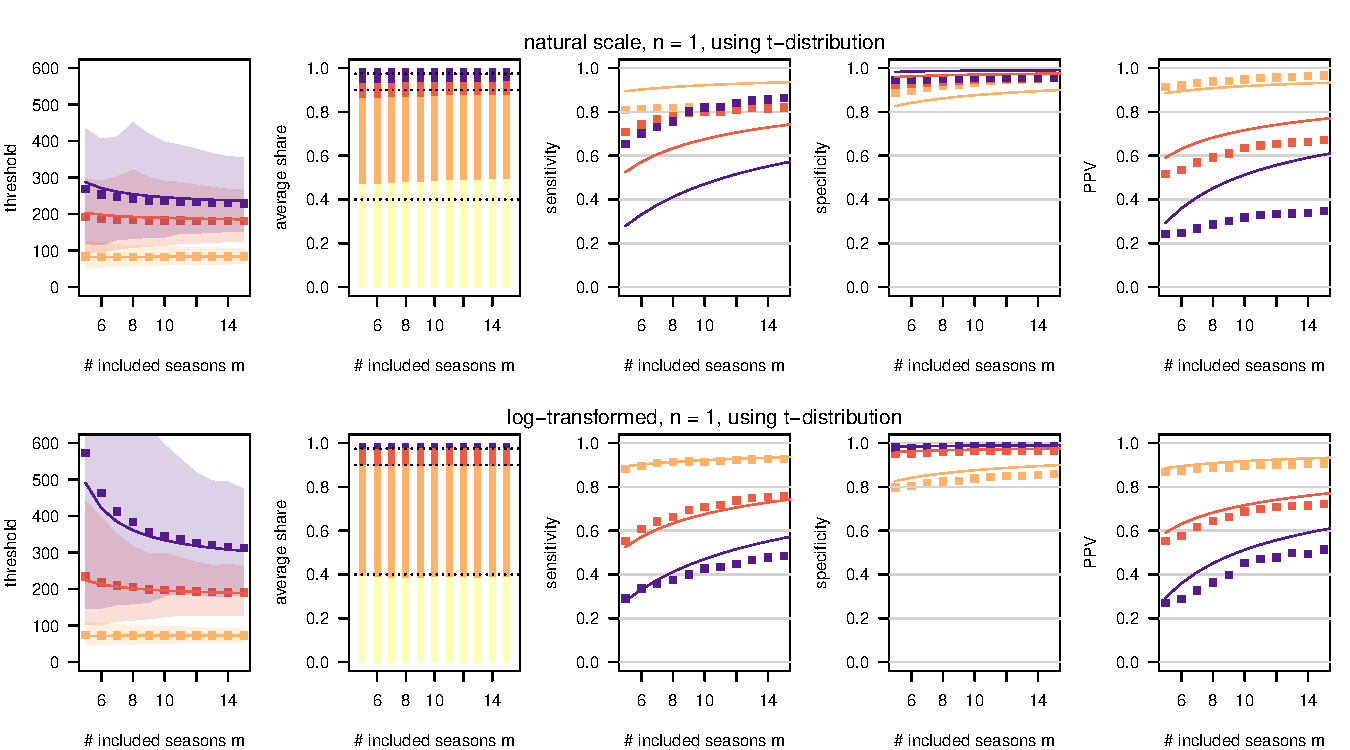
\includegraphics[width = 0.9\textwidth]{figure/plot_t_fr_small.pdf}\vspace{-5mm}
\end{center}
\caption{Summary of simulation results when thresholds are based on $t$ rather than normal distributions. See caption of Figure \ref{fig:results1} for details on the plot elements.}
\label{fig:t}
\end{figure}

\subsubsection{Accounting for secular trends}
\label{subsec:results_trends}

\textbf{Adapted simulation setup.} To assess thresholds which account for secular trends (settings g--h from Section \ref{subsec:simulation_setup}) we modify our simulation setting and artificially introduce such trends. To mimic an annual growth rate $r$, we multiply the values $x_{j, k}$ for seasons $j = 1, \dots, m + 1$ by $(1 + r)^{-(m + 1 - j)}$, respectively. The $m + 1$-th season remains unaffected by this modification and still follows the same distribution as in the previous sections. The seasons $1, \dots, m$ are characterized by a geometric trend approaching the usual level from above or below. For our simulation we consider $r = \pm 3\%$ and $\pm 7\%$, computing thresholds with and without a correction for secular trends. In all cases we use a logarithmic transformation and $n = 1$ along with a $t$-distribution.

\noindent \textbf{Thresholds and threshold exceedance.} Figure \ref{fig:trend} shows that ignoring secular trends leads to mis-calibrated thresholds, with stronger miscalibration for larger $m$. This is expected as seasons far in the past in expectation differ more strongly from the upcoming $(m + 1)$-th one. Thresholds corrected for secular trends using model \eqref{eq:trend} are well-calibrated. However, due to the addition of a parameter, the threshold values get considerably more variable. The corresponding display for $r = \pm 7\%$ is available in Supplementary Figure S5 and shows the same qualitative patterns.

\begin{figure}
\begin{center}
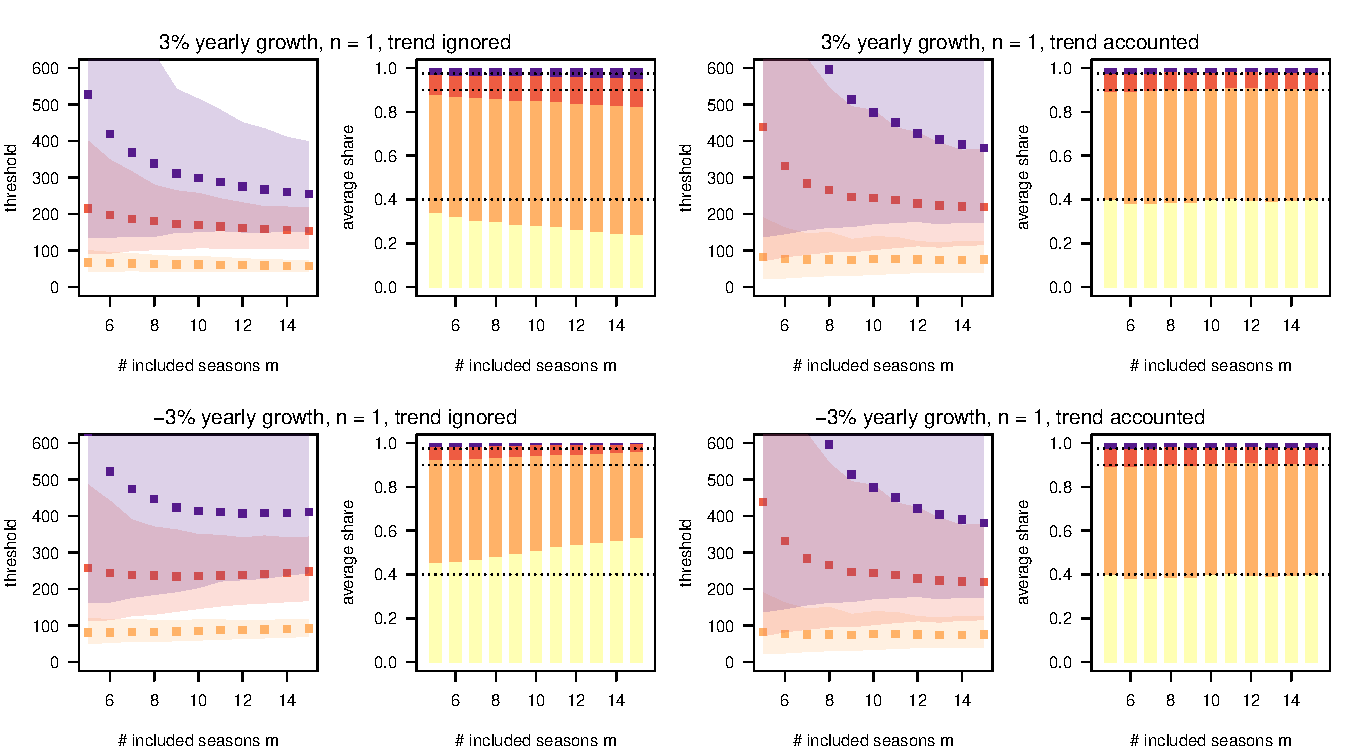
\includegraphics[width = 0.9\textwidth]{figure/plot_trend3_fr_small.pdf}\vspace{-5mm}
\end{center}
\caption{Average thresholds and exceedance shares in the presence of constant annual growth (3\%) and decrease (-3\%). In each setting we computed thresholds with and without accounting for the secular trend. See the caption and legend of Figure \ref{fig:results1} for details on the plot elements.}
\label{fig:trend}
\end{figure}

The sensitivity, specificity and positive predictive values of models with and without secular trends in different settings are compared in Supplementary Figure S6. If there is no true secular trend ($r = 0$), the inclusion of a superfluous trend parameter substantially decreases all three performance metrics, most strongly for small $m$. For the considered values of $m$, five to ten additional observations seem to be necessary to even out the cost of increased complexity. As suspected by \cite{Vega2013}, if secular trends are present but not accounted for, the performance of thresholds can decrease from a certain value of $m$ onwards. Little surprisingly, sensitivity will be compromised in case of downward trends, while upward trends hamper specificity and PPVs.

\noindent \textbf{When is it beneficial to correct thresholds for secular trends?} In many cases (consider e.g., PPVs for $r = 3\%$), accounting for trends in thresholds only pays off from a certain value of $m$ onwards. However, it is difficult to provide general guidance on when to trade the bias resulting from ignoring a secular trend for the increased estimation variability resulting from an additional parameter. A heuristic recommendation we can draw from Figures \ref{fig:trend} and Supplementary Figure S5 is that thresholds accounting for trends are extremely variable for $m < 10$. As discussed before, such high variability also implies that the high and very high thresholds need to be higher in expectation in order to be calibrated. This pattern is very pronounced in our examples. From $m = 10$, or better $m = 15$ onwards, thresholds are better-behaved. This finding should be taken into account when deciding on the inclusion of a trend parameter, see also the Discussion section.


\subsubsection{Basing thresholds on confidence intervals}

Lastly we address thresholds based on confidence intervals (case i). Figure \ref{fig:cis} shows that these are not well-behaved. As suggested in Section \ref{subsec:cis}, the mean thresholds at different levels approach each other as $m$ grows. Overall, a very high fraction of seasons is classified as very high intensity.

\begin{figure}[h!]
\begin{center}
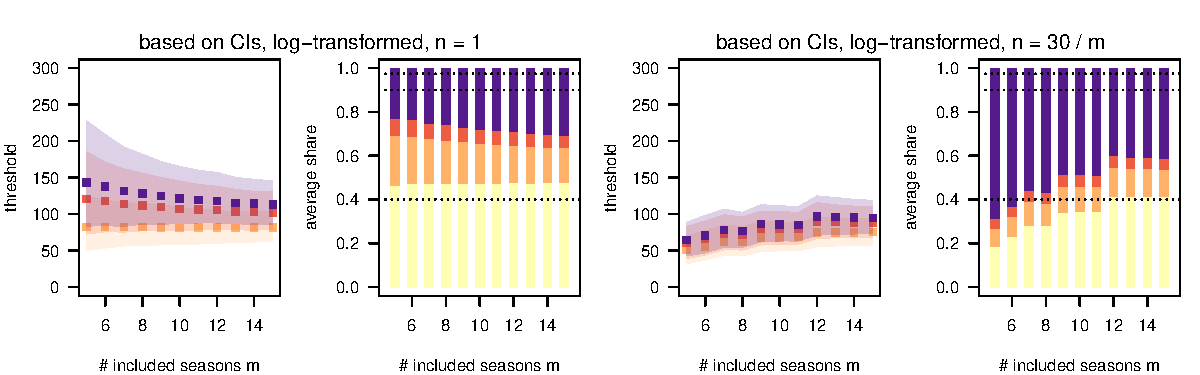
\includegraphics[width=0.9\textwidth]{figure/plot_ci_fr.pdf}\vspace{-5mm}
\end{center}
\caption{Average thresholds and exceedance shares when thresholds are based on confidence interval limits rather than predictive quantiles. See the caption and legend of Figure \ref{fig:results1} for details on the plot elements.}
\label{fig:cis}
\end{figure}




\subsection{Short summary of results based on US data}
\label{subsec:results_us}

The results obtained using the US data, shown in Supplementary Section D, are in good agreement with those presented for France. While there are some differences in the exact values of exceedance probabilities, sensitivities etc., the overall patterns and conclusions are identical.

\section{Discussion}
\label{sec:discussion}

\textbf{Practical recommendation.} We provided a statistical assessment of implementation choices in a widely used framework for influenza intensity thresholding. Our practical recommendation in light of the theoretical and empirical findings is as follows. We suggest including $n = 1$ observation per season into the reference set, employing a log transformation and basing thresholds on a $t$ rather than a normal distribution. A code snippet to apply these settings in the R package \texttt{mem} is available in Supplement B.1.

To make thresholds less variable, data can be smoothed using a moving average with $l = 3$. If smoothing is employed, the resulting thresholds should be applied to new data smoothed using the same procedure. Given the cost of estimating an extra parameter from limited data, our preliminary recommendation is that secular trends should only be accounted for if (a) this is supported by convincing epidemiological reasons and (b) data on at least $m = 10$ to 15 seasons is available.


\noindent \textbf{Summary in terms of desirable properties from Section \ref{sec:desirable_properties}.} For a more detailed conclusion we return to the criteria evoked in Section \ref{sec:desirable_properties}.

\begin{description}
\item \textbf{Calibration.} The key to well-calibrated thresholds is comparability of the reference set and new season peaks. This implies that no historical non-peak values should be included (i.e., one should choose $n = 1$). Otherwise thresholds will be pulled downwards and exceeded too frequently by new peaks. If historical data are smoothed ($l > 1$), comparability should be ensured by applying the same smoothing to new season peaks. Otherwise thresholds will again be exceeded too often. If the reference set only contains few values, thresholds should be based on quantiles of a $t$ rather than a normal distribution. Empirically we found that thresholds computed on log-transformed observations were better calibrated. We expect this to translate to other settings as distributions of peak values are typically skewed.\\
Discussions with public health experts showed that, based on practical use over the years, at least some were aware of the the miscalibration of the MEM and WHO methods. These analysts took the bias towards higher categories implicitly into account in their interpretation.
\item \textbf{Sensitivity and specificity.} Our theoretical and empirical results show that even under ideal conditions, the sensitivity and positive predictive values of thresholds cannot be expected to exceed rather modest levels if $m$ is small. This is unaffected by whether smoothing is applied and reflects the general difficulty of estimating extreme quantiles from few observations. Especially for the very high threshold at $\alpha = 0.975$, sensitivity and PPV must be expected to be modest and it can be asked whether these thresholds are practically meaningful. In any case it does not seem advisable to add even more extreme thresholds to the procedure. This problem is reduced if many historical seasons are available, but in practice there may be a tradeoff with the recency and comparability of these data. Secular trends in the data can be accounted for, which may enable the use of longer historical time series. However, the addition of a parameter also makes thresholds more variable.
\item \textbf{Stability.} The same difficulties limiting the sensitivity and PPV imply that thresholds are rather variable if $m$ is small. Empirically we found that this is even more the case if a log transformation is employed and if secular trends are accounted for. Smoothing of historical data reduces the variability of thresholds, but without improving sensitivity or specificity.
\item \textbf{Simplicity.} From a statistical standpoint the MEM and WHO methods are straightforward. However, exchange with users from public health indicates that given the large number of possible configurations, both methods are perceived as rather complex. Our subjective opinion is that the methods overall strike a good balance here. However, more specific guidance on how to choose the parameters of the methods and sensible default values is important to enable successful use of the methods. We note that a somewhat more sophisticated approach based on generalized additive models (GAMs) has recently been suggested \citep{Pang2023}.
\item \textbf{Ease of practical application.} Both methods can be applied using graphical user interfaces and thus do not require programming knowledge. For the MEM this is set up on top of an open-source R package with excellent documentation. For technically versed users we recommend using this package. Combined with minimal data pre-processing it covers most aspects discussed in this paper and enhances the automation and reproducibility of computations.
\end{description}

\noindent \textbf{Further discussion and outlook.} As evoked in the introduction, intensity thresholds are not only used to classify season peaks retrospectively, but also to assess intensity in real time in a weekly rhythm. In this setting, the MEM and WHO thresholds may not be very informative as they are designed for peak incidences and will rarely be exceeded early on in a season. Thresholds which, following the idea of the Serfling method, are specific to calendar weeks or weeks since season onset may be more suitable. Indeed, such an approach has been used to derive intensity thresholds for deaths due to pneumonia and influenza in \cite{Biggerstaff2017}. In discussions with public health experts, however, it was remarked that due to the variable season timing of influenza, the underlying idea of ``average seasonal shape'' may often not be adequate.

An alternative approach used e.g., in Singapore \citep{Pung2020} and previously the UK \citep{Green2015} is to use thresholds which do not vary over time, but nonetheless use \textit{all} historical observations rather than just peak or near-peak weeks as the reference (this corresponds essentially to using $n = 52$). This may be an attractive option especially in tropical regions with less stable seasonal influenza patterns. However, it changes the interpretation of thresholds. Exceedance probabilities then no longer refer to season peaks, but the entirety of weekly observations, which may be deemed more suitable for weekly real-time assessements.

In a similar fashion, the exceedance probabilities of the default MEM setting with $n > 1$ could be seen to refer to observations which are among the top $n$ of a season. We argue, however, that this interpretation lends itself less easily to season peak intensity classification as there would need to be an aggregation rule mapping the $n$ individual results to an overall category. Smoothing ($l > 1$) has a similar effect on thresholds, but implies a straightforward overall classification for a season.


On a more general note, it can be asked whether a categorization into four categories is the most appropriate way of conveying influenza activity. As evoked in Section \ref{subsubsec:n}, the highest season peaks from one category and the lowest from the one above are not qualitatively different. A discrete categorization may thus seem arbitrary and discards a lot of information. An alternative is to report which percentile of the fitted reference distribution a new peak reached, as previously done in certain countries \citep{Green2015}. This would result in a continuous scale from 0 to 100, with higher values indicating higher intensity. However, given the difficulties with estimating extreme quantiles, a percentile-based display may convey a false sense of exactness. In discussions with users from public health, it was moreover pointed out that the purpose of intensity classification was precisely to make high-level statements which are easy to communicate to decision makers and the public. In practice, a continous rating would again need to be translated to an appropriately named category, with the same issues as discussed above.

A fundamental difficulty of intensity thresholding lies in the estimation of extreme quantiles from limited data. The estimation of extreme quantiles is well-studied in extreme value theory, but even sample sizes considered small in this field exceed what is usually available for intensity thresholding (see e.g., \citealt{Pisarenko2017} who consider sample sizes of 50 to 100). To meaningfully improve thresholding, it thus seems necessary to integrate additional information. Bayesian approaches may be suitable to incorporate prior knowledge and thus regularize thresholds. Also, it may be possible to share statistical strength across different geographies. For the French data, exploratory analyses showed that after logarithmic transformation, the variability of peak values was similar within each region. Pooling information across regions may thus lead to better-behaved thresholds than when treating each region independently.




\noindent \textbf{Limitations.} The present study focuses on the statistical properties of thresholding methods, but we emphasize that intensity classification also requires in-depth domain knowledge. Indeed, some experts we consulted stated that in their institutions weekly classifications for international reports were occasionally overruled manually if there was reason to believe that current data were biased in a specific way. This illustrates that while statistical methods should of course be well-behaved, they are only one element in a more complex assessment process.

Moreover, some methodological and technical questions remain. For instance, it is straightforward to adjust thresholds for secular trends. In our discussions, public health experts overall considered it desirable to do so, especially if trends are assumed to be due to changes in reporting practices rather than actual incidence. However, it is unclear under which circumstances it is statistically advisable to include a trend parameter. In lack of a clear statistical criterion, our preliminary recommendation is to include a trend if epidemiological background knowledge supports this choice, but otherwise stick with a more parsimonious model excluding a trend. If an exceptionally long historical time series such as in the French example is available, a trend parameter can be more easily incorporated. In our simulation study, it appeared that from $m = 10$ to 15 onward, thresholds accounting for trends become better-behaved.

A related, but even more challenging question is how to address structural breaks in surveillance time series, as recently caused by the COVID-19 pandemic. A regression-based approach similar to \eqref{eq:trend} could be used to account for a shift in overall incidence levels. However, this would nonetheless require several years of post-pandemic data, and it is unclear if the implicit assumption of constant variance $\sigma^2_\varepsilon$ is justified. Also, it is unclear how extreme seasons in the historical data should be handled. These can have a substantial effect on thresholds. In our simulation study we pragmatically removed observations from the pandemic season 2009/2010, as done in \cite{Vega2015} and the \textit{WHO Average Curves} Shiny Web App default settings. However, a more principled approach to determine which historical seasons should be excluded would be desirable. As the same problem arises in outbreak detection, this strand of literature may be a helpful starting point (see e.g., \citealt{Noufaily2013}).



A limitation of our simulation study is that the re-sampled data do not actually stem from one and the same time series, but from several different regions. This made some re-scaling necessary. Also, dependence structures across seasons are not preserved, meaning that we cannot assess violations of assumption (HB) and (IB). A realistic correlation structure between season peaks and the surrounding values, however, is preserved, which would be challenging with fully synthetic data. We re-ran all simulation studies using a smaller data set from the United States and obtained very similar results. We take this as a sign of robustness at least for temperate settings. Intensity thresholds in tropical regions pose specific challenges like seasons with multiple peaks, which we did not address in the present manuscript.

\noindent \textbf{Conclusion.} To conclude, we re-emphasize the importance of a simple and interpretable thresholding method with a thorough open source software implementation like \texttt{mem}. The use of a standard approach will improve comparability of results and facilitate further methodological advances. With this work we hope to contribute to the development of best practices  with a statistical perspective, complementing public health practitioners' applied experience.

\paragraph{Data and code:} Materials to reproduce the presented results are available at \url{https://github.com/jbracher/mem_who}.

\paragraph{Ethics statement:} No ethics approval was necessary as this study uses exclusively publicly available data.

\paragraph{Copyright information for Figure \ref{fig:maps}:}

Top: Materials developed by CDC and available in the public domain (\url{https://www.cdc.gov/other/agencymaterials.html}). The use of this material in the present paper does not imply any endorsement by CDC, ATSDR, HHS or the United States Government. The materials are available free of charge from the CDC website. Bottom: Copyright European Centre for Disease Prevention and Control (\url{https://www.ecdc.europa.eu/en/copyright}). Information and documents made available on ECDC web pages and for which ECDC owns the copyright are public and may be reproduced, adapted and/or distributed, totally or in part, irrespective of the means and/or the formats used, provided that ECDC is always acknowledged as the original source of the material. Such acknowledgement must be included in each copy of the material. The use of this material in the present paper does not imply any endorsement by ECDC.

% \section*{Author contributions}

% Study concept: JB; Data processing: JB and JL; Literature review: JB and JL; Statistical analysis / implementation: JB; Writing and editing: JB and JL.


\paragraph{Acknowledgements:}

We would like to thank Matthew Biggerstaff, Sebastian Funk, Michael H\"ohle, Rob Moss, Rachael Pung, Alexander Ullrich, Laura Werlen and Daniel Wolffram for helpful discussions. Special thanks go to Jos\'e Eugenio Lozano and Tom\'as Vega, who extended the functionality of the \texttt{mem} package to include thresholds based on the $t$-distribution. Johannes Bracher was supported by the Helmholtz Foundation via the SIMCARD Information and Data Science Pilot Project as well as Deutsche Forschungsgemeinschaft (DFG, German Research Foundation) -- project number 512483310.

{\footnotesize
\bibliographystyle{apalike}
\bibliography{bibliography_mem}
}


\end{document}